% presentation
\documentclass{beamer}
\usetheme[height=7mm]{Rochester}
\usecolortheme{rose}

% handout

%\documentclass[handout]{beamer}
%\usepackage{pgfpages} \pgfpagesuselayout{8 on 1}[a4paper]

%\documentclass[mathserif]{article}
%\usepackage{beamerarticle}

\usepackage{amsmath}
\usepackage{comment}
\usepackage{amssymb,amsfonts}
\usepackage[T1]{fontenc}
\usepackage{lmodern}
\usepackage{tikz}
%\usepackage{simpsons}
\usepackage{marvosym}
\usepackage{color}
\usepackage{multirow}
\usepackage{pgffor}
\usepackage{pgfplots}
\usepackage[slide,algoruled,titlenumbered,vlined,noend,linesnumbered,]{algorithm2e}

\usefonttheme{structurebold}

\setbeamertemplate{footline}[frame number]
\setbeamertemplate{navigation symbols}{}
\setbeamerfont{smallverb}{size*={73}}
\usefonttheme[onlymath]{serif}
\setbeamertemplate{theorems}[numbered]
\newtheorem{construction}[theorem]{Construction}
\newtheorem{proposition}[theorem]{Proposition}

\AtBeginSection[] {
  \begin{frame}
    \frametitle{Content}
    \tableofcontents[currentsection]
  \end{frame}
  \addtocounter{framenumber}{-1}
}

\usetikzlibrary[shapes.arrows]
\usetikzlibrary{shapes.geometric}
\usetikzlibrary{backgrounds}
\usetikzlibrary{positioning}
\usetikzlibrary{calc}
\usetikzlibrary{intersections}
\usetikzlibrary{fadings}
\usetikzlibrary{decorations.footprints}
\usetikzlibrary{patterns}
\usetikzlibrary{shapes.callouts}
\usetikzlibrary{fit}
%handout

\providecommand{\abs}[1]{\lvert#1\rvert}

\tikzset{every picture/.style={line width=1pt,show background rectangle},background rectangle/.style={fill=blue!10,rounded corners=2ex}}

\newcommand{\Bob}[3]{ \begin{scope}[shift={(#1,#2)},scale=#3]
  \draw (0,0) circle (0.95 and 1);
  \fill (-0.3,-0.1) circle (0.1);
  \fill (+0.3,-0.1) circle (0.1);
  \draw (0.35,-0.5) arc (-70:-110: 1 and 0.4);
  \draw (-0.3,0.5) arc (-10:-80: 0.8 and 0.8);
  \draw (-0.5,0.8) arc (190:255: 2 and 1);
  \draw (-0.7,0.9) -- +(0.2,-0.09) -- +(0.25,0.2);
  \end{scope} }

\newcommand{\Alice}[3]{ \begin{scope}[shift={(#1,#2)},scale=#3]
  \draw (0,0) circle (0.95 and 1);
  \fill (-0.3,-0.1) circle (0.1);
  \fill (+0.3,-0.1) circle (0.1);
  \draw (0.35,-0.5) arc (-70:-110: 1 and 0.4);
  \draw (0.3,1.3) arc (20:-100: 1.4 and 1);
  \draw (0.5,1.3) arc (150:260: 1 and 1);
  \draw (0.41,1.3) circle (0.35);
  \end{scope} }

  \newcommand{\Evil}[3]{ \begin{scope}[shift={(#1,#2)},scale=#3]
    \draw (0,0) circle (0.95 and 1);
    \fill (-0.1,-0.1) -- +(-0.2,-0.1) -- +(-0.4,0.2); %eye
    \fill (0.1,-0.1) -- +(0.2,-0.1) -- +(0.4,0.2);
    \draw (0.35,-0.5) arc (-70:-110: 1 and 0.4);
    %\fill (0.3,-0.5) -- +(-0.1,-0.2) -- +(-0.2,-0.02);
    %\fill (-0.3,-0.5) -- +(0.1,-0.2) -- +(0.2,-0.02);
    \fill (0.3,0.7) -- +(0.5,0.4) -- +(0.4,-0.2); % horn
    \fill (-0.3,0.7) -- +(-0.5,0.4) -- +(-0.4,-0.2);
    %\draw (0.3,1.3) arc (20:-100: 1.4 and 1);
    %\draw (0.5,1.3) arc (150:260: 1 and 1);
    %\draw (0.41,1.3) circle (0.35);
    \end{scope} }

\newcommand{\Charlie}[3]{ \begin{scope}[shift={(#1,#2)},scale=#3]
    \draw (0,0) circle (0.95 and 1);
    \filldraw[fill=black!20] (-0.35,-0.1) circle (0.25);
    \filldraw[fill=black!20] (+0.35,-0.1) circle (0.25);
    %\draw (0.9,0.2) to [bend left] (-0.9,0.2);
    \draw (0.2,0) to [bend left] (-0.2,0);


    %\draw (0.3,0.7) to [bend right] (-0.3,0.7);
    %\draw (0.4,0.5) to [bend right] (-0.4,0.5);
    %\draw (0.35,-0.5) arc (-70:-110: 1 and 0.4);
    \draw (-0.7,-0.6) to [bend right] (0,-0.6) to [bend right] (0.7,-0.6) to [bend right]  (0,-0.5)  to [bend right]  cycle ;
    %\draw (0.3,1.3) arc (20:-100: 1.4 and 1);
    %\draw (0.5,1.3) arc (150:260: 1 and 1);
    %\draw (0.41,1.3) circle (0.35);
    \end{scope} }

\author{Yu Zhang}
\institute{Harbin Institute of Technology}
\date[Crypto'22A]{Cryptography, Autumn, 2022}

%% presentation
\documentclass{beamer}
\usetheme[height=7mm]{Rochester}
\usecolortheme{rose}

% handout

%\documentclass[handout]{beamer}
%\usepackage{pgfpages} \pgfpagesuselayout{8 on 1}[a4paper]

%\documentclass[mathserif]{article}
%\usepackage{beamerarticle}

\usepackage{amsmath}
\usepackage{comment}
\usepackage{amssymb,amsfonts}
\usepackage[T1]{fontenc}
\usepackage{lmodern}
\usepackage{tikz}
%\usepackage{simpsons}
\usepackage{marvosym}
\usepackage{color}
\usepackage{multirow}
\usepackage{pgffor}
\usepackage{pgfplots}
\usepackage[slide,algoruled,titlenumbered,vlined,noend,linesnumbered,]{algorithm2e}

\usefonttheme{structurebold}

\setbeamertemplate{footline}[frame number]
\setbeamertemplate{navigation symbols}{}
\setbeamerfont{smallverb}{size*={73}}
\usefonttheme[onlymath]{serif}
\setbeamertemplate{theorems}[numbered]
\newtheorem{construction}[theorem]{Construction}
\newtheorem{proposition}[theorem]{Proposition}

\AtBeginSection[] {
  \begin{frame}
    \frametitle{Content}
    \tableofcontents[currentsection]
  \end{frame}
  \addtocounter{framenumber}{-1}
}

\usetikzlibrary[shapes.arrows]
\usetikzlibrary{shapes.geometric}
\usetikzlibrary{backgrounds}
\usetikzlibrary{positioning}
\usetikzlibrary{calc}
\usetikzlibrary{intersections}
\usetikzlibrary{fadings}
\usetikzlibrary{decorations.footprints}
\usetikzlibrary{patterns}
\usetikzlibrary{shapes.callouts}
\usetikzlibrary{fit}
%handout

\providecommand{\abs}[1]{\lvert#1\rvert}

\tikzset{every picture/.style={line width=1pt,show background rectangle},background rectangle/.style={fill=blue!10,rounded corners=2ex}}

\newcommand{\Bob}[3]{ \begin{scope}[shift={(#1,#2)},scale=#3]
  \draw (0,0) circle (0.95 and 1);
  \fill (-0.3,-0.1) circle (0.1);
  \fill (+0.3,-0.1) circle (0.1);
  \draw (0.35,-0.5) arc (-70:-110: 1 and 0.4);
  \draw (-0.3,0.5) arc (-10:-80: 0.8 and 0.8);
  \draw (-0.5,0.8) arc (190:255: 2 and 1);
  \draw (-0.7,0.9) -- +(0.2,-0.09) -- +(0.25,0.2);
  \end{scope} }

\newcommand{\Alice}[3]{ \begin{scope}[shift={(#1,#2)},scale=#3]
  \draw (0,0) circle (0.95 and 1);
  \fill (-0.3,-0.1) circle (0.1);
  \fill (+0.3,-0.1) circle (0.1);
  \draw (0.35,-0.5) arc (-70:-110: 1 and 0.4);
  \draw (0.3,1.3) arc (20:-100: 1.4 and 1);
  \draw (0.5,1.3) arc (150:260: 1 and 1);
  \draw (0.41,1.3) circle (0.35);
  \end{scope} }

  \newcommand{\Evil}[3]{ \begin{scope}[shift={(#1,#2)},scale=#3]
    \draw (0,0) circle (0.95 and 1);
    \fill (-0.1,-0.1) -- +(-0.2,-0.1) -- +(-0.4,0.2); %eye
    \fill (0.1,-0.1) -- +(0.2,-0.1) -- +(0.4,0.2);
    \draw (0.35,-0.5) arc (-70:-110: 1 and 0.4);
    %\fill (0.3,-0.5) -- +(-0.1,-0.2) -- +(-0.2,-0.02);
    %\fill (-0.3,-0.5) -- +(0.1,-0.2) -- +(0.2,-0.02);
    \fill (0.3,0.7) -- +(0.5,0.4) -- +(0.4,-0.2); % horn
    \fill (-0.3,0.7) -- +(-0.5,0.4) -- +(-0.4,-0.2);
    %\draw (0.3,1.3) arc (20:-100: 1.4 and 1);
    %\draw (0.5,1.3) arc (150:260: 1 and 1);
    %\draw (0.41,1.3) circle (0.35);
    \end{scope} }

\newcommand{\Charlie}[3]{ \begin{scope}[shift={(#1,#2)},scale=#3]
    \draw (0,0) circle (0.95 and 1);
    \filldraw[fill=black!20] (-0.35,-0.1) circle (0.25);
    \filldraw[fill=black!20] (+0.35,-0.1) circle (0.25);
    %\draw (0.9,0.2) to [bend left] (-0.9,0.2);
    \draw (0.2,0) to [bend left] (-0.2,0);


    %\draw (0.3,0.7) to [bend right] (-0.3,0.7);
    %\draw (0.4,0.5) to [bend right] (-0.4,0.5);
    %\draw (0.35,-0.5) arc (-70:-110: 1 and 0.4);
    \draw (-0.7,-0.6) to [bend right] (0,-0.6) to [bend right] (0.7,-0.6) to [bend right]  (0,-0.5)  to [bend right]  cycle ;
    %\draw (0.3,1.3) arc (20:-100: 1.4 and 1);
    %\draw (0.5,1.3) arc (150:260: 1 and 1);
    %\draw (0.41,1.3) circle (0.35);
    \end{scope} }

\author{Yu Zhang}
\institute{Harbin Institute of Technology}
\date[Crypto'22A]{Cryptography, Autumn, 2022}

%\input{1introduction.tex}
%\input{2perfectlysecret.tex}
%\input{3privatekey.tex}


\title{Introduction}

\begin{document}
\maketitle
\begin{frame}
\frametitle{Outline}
\tableofcontents
\end{frame}
\section{Cryptography and Modern Cryptography}
\begin{frame}\frametitle{What is Cryptography?}
\begin{itemize}
\item \textbf{Cryptography}: from Greek \emph{krypt\'os}, ``hidden, secret''; and \emph{gr\'{a}phin}, ``writing''
\item \textbf{Cryptography}: the art of writing or solving codes.\\ (Concise oxford dictionary 2006)
\item \textbf{Codes}: a system of prearranged signals, especially used to ensure secrecy in transmitting messages. \\ (\emph{code word} in cryptography)
\item \textbf{1980s}: from Classic to Modern; from Military to Everyone
\item \textbf{Modern cryptography}: the scientific study of mathematical techniques for securing digital information, systems, and distributed computations against adversarial attacks
\end{itemize}
\end{frame}
\begin{frame}\frametitle{What is cryptography? [xkcd:504]}
\begin{figure}
\begin{center}
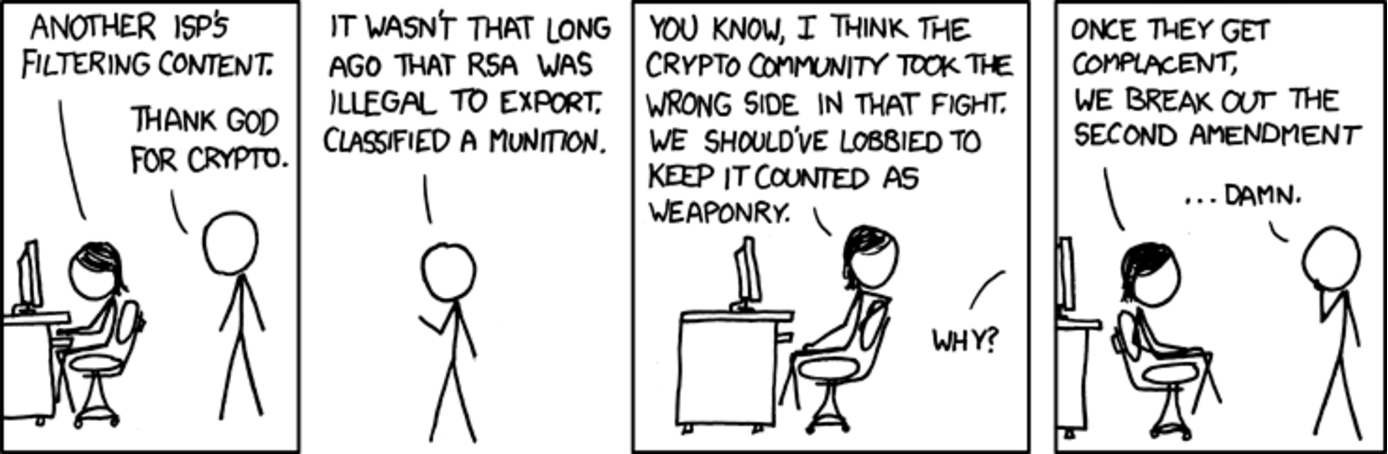
\includegraphics[width=100mm]{pic/legal} 
\end{center}
\end{figure}
\end{frame}
\section{The Setting of Private-Key Encryption}
\begin{frame}\frametitle{Private-Key Encryption}
\begin{itemize}
\item \textbf{Goal}: to construct \textbf{ciphers} (encryption schemes) for providing secret communication between two parties sharing \textbf{private-key} (the symmetric-key) in advance
\item \textbf{Implicit assumption}: there is some way of initially sharing a key in a secret manner
\item \textbf{Disk encryption}: the same user at different points in time
\end{itemize}
\end{frame}
\begin{frame}\frametitle{Alice, Bob  [xkcd:1323]}
Changing the names would be easier, but if you're not comfortable lying, try only making friends with people named Alice, Bob, Carol, etc.
\begin{figure}
\begin{center}
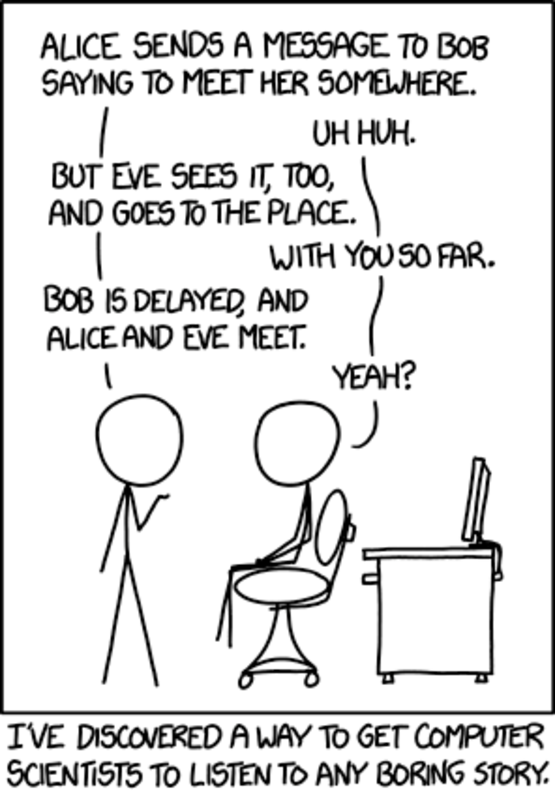
\includegraphics[width=45mm]{pic/alice-bob} 
\end{center}
\end{figure}
\end{frame}
\begin{frame}\frametitle{The Syntax of Encryption}
\begin{figure}
\begin{center}
\begin{tikzpicture}
\node (sender) [minimum size=1cm] {}; \Alice{0}{0}{0.4};
\node (bart) [below of = sender, node distance = 0.7cm] {Alice};
\node (enc) [draw, right of = sender, rounded corners=1ex,node distance = 2cm] {$\mathsf{Enc}$};
\node (k1) [above of = enc, node distance = 1cm] {$k$};
\node (c) [right of = enc, node distance = 2cm] {$c$};
\node (gen) [draw, above of = c, rounded corners=1ex,node distance = 1cm] {$\mathsf{Gen}$};
\node (adv) [below of = c, node distance = 1cm, minimum size=1cm] {}; \Evil{4cm}{-1cm}{0.4};
\node (burns) [below of = adv, node distance = 0.7cm] {Adversary};
\node (dec) [draw, right of = c, rounded corners=1ex,node distance = 2cm] {$\mathsf{Dec}$};
\node (k2) [above of = dec, node distance = 1cm] {$k$};
\node (receiver) [right of = dec, node distance = 2cm, minimum size=1cm] {}; \Bob{8cm}{0}{0.4};
\node (lisa) [below of = receiver, node distance = 0.7cm] {Bob};
\draw[-latex] (sender) -- (enc) node [midway, above] {$m$};
\draw (enc) -- (c); \draw[-latex] (c) -- (dec);
\draw[-latex] (dec) -- (receiver) node [midway, above] {$m$};
\draw[-latex] (k1) -- (enc);
\draw[-latex] (gen) -- (k1);
\draw[-latex] (gen) -- (k2);								
\draw[-latex] (k2) -- (dec);		
\end{tikzpicture}
\end{center}
\end{figure}
\begin{itemize}
\item key $k \in \mathcal{K}$, plaintext (or message) $m \in \mathcal{M}$, ciphertext $c \in \mathcal{C}$
\item \textbf{Key-generation} algorithm~$k \gets \mathsf{Gen}$
\item \textbf{Encryption} algorithm~$c:= \mathsf{Enc}_k(m)$
\item \textbf{Decryption} algorithm~$m:= \mathsf{Dec}_k(c)$
\item \textbf{Encryption scheme}: $\Pi = (\mathsf{Gen}, \mathsf{Enc}, \mathsf{Dec})$
\item \textbf{Basic correctness requirement}: $\mathsf{Dec}_k(\mathsf{Enc}_k(m)) = m$
\end{itemize}
\end{frame}
\begin{frame}\frametitle{Securing Key vs Obscuring Algorithm}
\begin{itemize}
\item Easier to maintain secrecy of a short key
\item In case the key is exposed, easier for the honest parties to change the key
\item In case many pairs of people, easier to use the same algorithm, but different keys
\end{itemize}
\begin{alertblock}{Kerckhoffs's principle}
\begin{quote}
The cipher method must not be required to be secret, and it must be able to fall into the hands of the enemy without inconvenience.
\end{quote}	
\end{alertblock}
\begin{alertblock}{Shannon's maxim}
	\begin{quote}
		The enemy knows the system.
	\end{quote}	
\end{alertblock}
\end{frame}
\begin{frame}\frametitle{Why ``Open Cryptographic Design''}
\begin{itemize}
\item Published designs undergo public scrutiny are to be stronger
\item Better for security flaws to be revealed by ``ethical hackers''
\item Reverse engineering of the code (or leakage by industrial espionage) poses a serious threat to security
\item Enable the establishment of standards.
\end{itemize}
\begin{exampleblock}{Dual EC: A Standardized Back Door}
	``Dual EC was standardized by NIST, ANSI, and ISO among other algorithms to generate pseudorandom numbers.'' ``The Snowden revelations, and in particular reports on Project Bullrun and the SIGINT Enabling Project, have indicated that Dual EC was part of a systematic effort by NSA to subvert standards.'' ``Reuters reported that NSA paid RSA ``\$10 million in a deal that set [Dual EC] as the preferred, or default, method for number generation in the BSafe software.''''	
\end{exampleblock}
\end{frame}
\begin{frame}\frametitle{Attack Scenarios}	
\begin{itemize}
\item \textbf{Ciphertext-only}: the adversary just observes ciphertext
\item \textbf{Known-plaintext}: the adversary learns pairs of plaintexts/ciphertexts under the same key
\item \textbf{Chosen-plaintext}: the adversary has the ability to obtain the encryption of plaintexts of its choice
\item \textbf{Chosen-ciphertext}: the adversary has the ability to obtain the decryption of \textbf{other} ciphertexts of its choice
\item \textbf{Passive attack}: COA KPA
\begin{itemize}
\item because not all ciphertext are confidential
\end{itemize}
\item \textbf{Active attack}: CPA CCA
\begin{itemize}
\item when to encrypt/decrypt whatever an adversary wishes?
\end{itemize}
\end{itemize}	
\end{frame}
\section{Historical Ciphers and Their Cryptanalysis}
\begin{comment}
	\begin{frame}\frametitle{Why We Learn Broken Ciphers?}
	\begin{itemize}
	\item To understand the weaknesses of an ``ad-hoc'' approach
	\item To learn that ``simple'' approaches are unlikely to succeed
	\item To feel that ``we are smart enough to do some crypt-analyzing''
	\end{itemize}
	\end{frame}
\end{comment}

\begin{frame}[fragile]\frametitle{Caesar's Cipher}
\begin{quote}
If he had anything confidential to say, he wrote it in cipher, that is, by so changing the order of the letters of the alphabet, that not a word could be made out. If anyone wishes to \alert{decipher} these, and get at their meaning, he must \alert{substitute the fourth letter of the alphabet, namely D, for A}, and so with the others

\rightline{--Suetonius,``Life of Julius Caesar''}
\end{quote}
\begin{itemize}
	\item $\mathsf{Enc}(m)=m+3\mod 26$ \footnote{In fact the quote indicates that decryption involved rotating letters of the alphabet forward 3 positions, $\mathsf{Dec}(c)=c+3\mod 26$}
	\item \textbf{Weakness}: ? %\alert{What is the key?}
\end{itemize}
\begin{exampleblock}{Example}
\verb|begintheattacknow|
%\verb|EHJLQWKHDWWDFNQRZ|
\end{exampleblock}
\end{frame}
\begin{frame}[fragile]\frametitle{Shift Cipher}
\begin{itemize}
\item $\mathsf{Enc}_k(m)=m+k\mod 26$
\item $\mathsf{Dec}_k(c)=c-k\mod 26$
\item \textbf{Weakness}: ? %Fragile under \textbf{Brute-force attack} (exhaustive search)
\end{itemize}
\begin{exampleblock}{Example: Decipher the string}	
\verb|EHJLQWKHDWWDFNQRZ|
\end{exampleblock}
\begin{alertblock}{Sufficient Key Space Principle}
Any secure encryption scheme must have a key space that is not vulnerable to exhaustive search.\footnote{If the plaintext space is larger than the key space.}
\end{alertblock}
\end{frame}
\begin{frame}\frametitle{Index of Coincidence (IC) Method (to find $k$)}
\textbf{How to automatically determine that the deciphered text makes sense?}

\textbf{Index of Coincidence (IC)}: the probability that two randomly selected letters (pick-then-return) will be identical.

Let $p_i$ denote the probability of $i$th letter in English text.
\[I \overset{\text{def}}{=}\sum_{i=0}^{25} p_i^2 \]
\begin{exampleblock}{Example}
What's the IC of `apple'?
\end{exampleblock}

For a long English text, the IC is $\approx 0.065$.
For $j = 0, 1, \dotsc , 25$, $q_j$ is the probability of $j$th letter in the ciphertext.
\[I_j \overset{\text{def}}{=}\sum_{i=0}^{25} p_i \cdot q_{i+j}\]
\alert{Q: For shift cipher, if $j = k$, then $I_j \approx$ ?}
\end{frame}

\begin{frame}[fragile]\frametitle{Mono-Alphabetic Substitution}
\begin{itemize}
\item \textbf{Idea}: To map each character to a different one in an arbitrary manner
\item \textbf{Strength}: Key space is large $\approx 2^{88}$. \alert{Q: how to count?}
\item \textbf{Weakness}: ? %The mapping of each letter is fixed
\end{itemize}
\begin{exampleblock}{Example}
\verb|abcdefghijklmnopqrstuvwxyz|\\
\verb|XEUADNBKVMROCQFSYHWGLZIJPT|

Plaintext: \verb|tellhimaboutme|\\
Ciphertext: \verb|??????????????|
\end{exampleblock}
\end{frame}
\begin{frame}[fragile]\frametitle{Attack with Statistical Patterns}
\begin{enumerate}
\item Tabulate the frequency of letters in the ciphertext
\item Compare it to those in English text
\item Guess the most frequent letter corresponds to \verb|e|, and so on
\item Choose the plaintext that does ``make sense'' (Not trivial)
\end{enumerate}
\begin{table}
\begin{center}
\caption{Average letter frequencies for English-language text}
\begin{tabular}{|cc|cc|cc|cc|cc|} \hline
e & 12.7\% & t & 9.1\% & a & 8.2\% & o & 7.5\% & i & 7.0\%\\
n & 6.7\% & \_ & 6.4\% & s & 6.3\% & h & 6.1\% & r & 6.0\%\\
d & 4.3\% & l & 4.0\% & c & 2.8\% & u & 2.8\% & m & 2.4\%\\
w & 2.4\% & f & 2.2\% & g & 2.0\% & y & 2.0\% & p & 1.9\%\\
b & 1.5\% & v & 1.0\% & k & 0.8\% & j & 0.2\% & x & 0.2\%\\
q & 0.1\% & z & 0.1\% & & & & & &\\ \hline
\end{tabular}
\end{center}
\end{table}
\end{frame}
\begin{frame}[fragile]\frametitle{Example of Frequency Analysis (Ciphertext)}
\begin{verbatim}
LIVITCSWPIYVEWHEVSRIQMXLEYVEOIEWHRXEXIPFEMVEWHKVS
TYLXZIXLIKIIXPIJVSZEYPERRGERIMWQLMGLMXQERIWGPSRIH
MXQEREKIETXMJTPRGEVEKEITREWHEXXLEXXMZITWAWSQWXSWE
XTVEPMRXRSJGSTVRIEYVIEXCVMUIMWERGMIWXMJMGCSMWXSJO
MIQXLIVIQIVIXQSVSTWHKPEGARCSXRWIEVSWIIBXVIZMXFSJX
LIKEGAEWHEPSWYSWIWIEVXLISXLIVXLIRGEPIRQIVIIBGIIHM
WYPFLEVHEWHYPSRRFQMXLEPPXLIECCIEVEWGISJKTVWMRLIHY
SPHXLIQIMYLXSJXLIMWRIGXQEROIVFVIZEVAEKPIEWHXEAMWY
EPPXLMWYRMWXSGSWRMHIVEXMSWMGSTPHLEVHPFKPEZINTCMXI
VJSVLMRSCMWMSWVIRCIGXMWYMX
\end{verbatim}
\end{frame}
\begin{frame}[fragile]\frametitle{Example of Frequency Analysis (Analysis)}
Count and Guess, Trial and Error.
\begin{table}
\begin{center}
\caption{Analysis Steps}
\begin{tabular}{|r|l|} \hline
Ciphertext & Plaintext \\ \hline
\alert{I}   & \alert{e} \\
\alert{XLI} & \alert{the} \\
\alert{E} & \alert{a} \\
\alert{R}tate & \alert{s}tate \\
atthatt\alert{MZ}e & atthatt\alert{im}e \\
he\alert{V}e & he\alert{r}e \\
remar\alert{A} & remar\alert{k} \\ \hline
\end{tabular}
\end{center}
\end{table}
\end{frame}
\begin{frame}[fragile]\frametitle{Example of Frequency Analysis (Plaintext)}
\begin{quote}
Hereupon Legrand arose, with a grave and stately air, and brought me the beetle
from a glass case in which it was enclosed. It was a beautiful scarabaeus, and, at
that time, unknown to naturalists -- of course a great prize in a scientific point
of view. There were two round black spots near one extremity of the back, and a
long one near the other. The scales were exceedingly hard and glossy, with all the
appearance of burnished gold. The weight of the insect was very remarkable, and,
taking all things into consideration, I could hardly blame Jupiter for his opinion
respecting it.

\rightline{--Edgar Allan Poe's ``The Gold-Bug''}
\end{quote}
\end{frame}

\begin{frame}[fragile]\frametitle{Vigen\`{e}re (poly-alphabetic shift) Cipher}
\begin{itemize}
\item \textbf{Idea}: To ``smooth out'' the distribution in the ciphertext by mapping different instances of the same letter in the plaintext to different ones in the ciphertext
\item \textbf{Encryption}: $c_i=m_i+k_{[i\bmod t]}$, $t$ is the length (period) of $k$
\item \textbf{Cryptanalysis}: Need find $t$; if $t$ is known, need know whether the decryption ``makes sense'', but brute force ($26^t$) is infeasible for $t > 15$
\end{itemize}
\begin{exampleblock}{Example (Key is `cafe')}
\begin{description}[Ciphertext]
\item[Plaintext]  \verb|tellhimaboutme| \\
\item[Key]        \verb|cafecafecafeca| \\
\item[Ciphertext] \verb|??????????????| %\verb|WFRQKJSFEPAYPF|
\end{description}
\end{exampleblock}
\end{frame}
\begin{frame}[fragile]\frametitle{Kasiski's Method (to find $t$)}
\begin{itemize}
\item To identify repeated patterns of length 2 or 3
\item The distance between such appearances is a multiple of $t$
\item $t$ is the greatest common divisor of all the distances
\end{itemize}
\begin{exampleblock}{Example (Key is `beads')}
\begin{semiverbatim}
themanandthewomanretrievedtheletterfromthepostoffice
beadsbeadsbeadsbeadsbeadsbeansdeadsbeadsbeadsbeadbea
VMFQTPFOH\alert{MJJ}XSFCSSIMTNFZXFYISEIYUIKHWPQ\alert{MJJ}QSLVTGJKGF
\end{semiverbatim}
\end{exampleblock}
\end{frame}
\begin{frame}\frametitle{Index of Coincidence (IC) Method (to find $t$)}
For $\tau = 1, 2, \dotsc$, $q_i$ is the probability of $i$th letter in $c_1, c_{1+\tau}, c_{1+2\tau}, \dotsc$, IC is
\[I_\tau \overset{\text{def}}{=}\sum_{i=0}^{25} q_i^2\]
\alert{If $\tau = t$, then $I_\tau \approx ?$} ; otherwise $q_i \approx \frac{1}{26}$ and
\[I_\tau \approx \sum_{i=0}^{25} \left(\frac{1}{26}\right)^2 \approx 0.038\]
Then reuse IC method to find $k_i$.
\begin{alertblock}{Arbitrary Adversary Principle}
Security must be guaranteed for any adversary within the class of adversaries having the specified power
\end{alertblock}
\end{frame}
\begin{frame}\frametitle{Cryptanalytic Attacks (homework assignment)}
\begin{itemize}
\item Under COA, the requirement for ciphertext related to the size of the key space.  Vig\`{e}nere > mono-alphabetic sub. > shift
\item Under KPA, trivially broken.
\end{itemize}
\begin{alertblock}{Lessons learned}
\begin{itemize}
\item Sufficient key space principle
\item Designing secure cipher is a hard task
\item Complexity does not imply security (then what does?)
\item Arbitrary adversary principle
\end{itemize}
\end{alertblock}
\end{frame}
\section{The Basic Principles of Modern Cryptography}
\begin{frame}\frametitle{Three Main Principles of Modern Cryptography}
\begin{enumerate}
\item The formulation of a rigorous \textbf{definition} of security / threat model
\item When the security of a cipher relies on an unproven \textbf{assumption}, this assumption must be precisely stated and be as minimal as possible
\item Cipher should be accompanied by a rigorous \textbf{proof} of security with the above definition and the above assumption
\end{enumerate}
\end{frame}
\begin{frame}\frametitle{Why Principle 1 -- Formulation of Exact Definitions}
\begin{exampleblock}{Q: how would you formalize the security for private-key encryption?}
\begin{enumerate}
\item \emph{No adversary can find the secret key when given a ciphertext.}\\
$\mathsf{Enc}_k(m)=m$
\item \emph{No adversary can find the plaintext that corresponds to the ciphertext.}\\
$\mathsf{Enc}_k(m)=m_{0}\| \mathsf{AES}_k(m)$
\item \emph{No adversary can determine any character of the plaintext that corresponds to the ciphertext.}\\
$m=1000$, someone can learn $ 800 < m < 1200$
\item \emph{No adversary can derive any meaningful information about the plaintext from the ciphertext.}\\
Could you define so-called `meaningful'?
\end{enumerate}
\emph{\alert{Definitions of security should suffice for all potential applications.}}
\end{exampleblock}
\end{frame}
\begin{frame}\frametitle{Why Principle 1 -- How to define}
%\begin{exampleblock}{General Form}
%A cryptographic scheme for a given \textbf{task} is secure if no adversary of a specified \textbf{power} can achieve a specified \textbf{break}
%\end{exampleblock}

How To Define Security -- Lesson From Alan Turing
\begin{itemize}
\item What's computation?\footnote{Q: Any ``mathematical proof that there exist well-defined problems that computers cannot solve''? A: Halting Problem in computability theory}
\begin{enumerate}
\item A direct appeal to \textbf{intuition}
\item A \textbf{proof of the equivalence} of two definitions\\ (The new one has a greater intuitive appeal)
\item Giving \textbf{examples} solved using a definition
\end{enumerate}
\item Additional method for security: \textbf{Test of time}
\end{itemize}
\end{frame}	
\begin{frame}\frametitle{Principle 2 -- Reliance on Precise Assumptions}
Most cryptographic constructions \textbf{cannot be proven secure unconditionally}
\begin{itemize}
	\item \textbf{Why?} 
	\begin{enumerate}
		\item Validation of the assumption
		\item Comparison of schemes
		\item Facilitation of proofs of security
	\end{enumerate}
	\textbf{The construction is secure if the assumption is true.}
	\item \textbf{How?} 
	\begin{enumerate}
		\item old, so well tested
		\item simple and lower-level, so easy to study, refute \& correct
	\end{enumerate}
\end{itemize}
\end{frame}
\begin{frame}\frametitle{Principle 3 -- Rigorous Proofs of Security}
\begin{itemize}
\item \textbf{Why?} Proofs are more desirable in computer security than in other fields.
\item \textbf{The reductionist approach}: 
\begin{theorem}	Given that Assumption X is true, Construction Y is secure according to the given definition.
\end{theorem}
\begin{proof} Reduce the problem given by X to the problem of breaking Y.
\end{proof}
\item \textbf{Ad-hoc approaches}: for those who need a ``quick and dirty'' solution, or who are just simply unaware.
\end{itemize}
\end{frame}
\begin{frame}\frametitle{Summary}
\begin{itemize}
\item Cryptography secures information, transactions and computations
\item Kerckhoffs's principle \& Open cryptographic design
\item Caesar's, shift, Mono-Alphabetic sub., Vigen\`{e}re
\item Brute force, letter frequency, Kasiski's, IC
\item Sufficient key space principle
\item Arbitrary adversary principle
\item Rigorously proven security
\end{itemize}
\end{frame}
\end{document}


%% presentation
\documentclass{beamer}
\usetheme[height=7mm]{Rochester}
\usecolortheme{rose}

% handout

%\documentclass[handout]{beamer}
%\usepackage{pgfpages} \pgfpagesuselayout{8 on 1}[a4paper]

%\documentclass[mathserif]{article}
%\usepackage{beamerarticle}

\usepackage{amsmath}
\usepackage{comment}
\usepackage{amssymb,amsfonts}
\usepackage[T1]{fontenc}
\usepackage{lmodern}
\usepackage{tikz}
%\usepackage{simpsons}
\usepackage{marvosym}
\usepackage{color}
\usepackage{multirow}
\usepackage{pgffor}
\usepackage{pgfplots}
\usepackage[slide,algoruled,titlenumbered,vlined,noend,linesnumbered,]{algorithm2e}

\usefonttheme{structurebold}

\setbeamertemplate{footline}[frame number]
\setbeamertemplate{navigation symbols}{}
\setbeamerfont{smallverb}{size*={73}}
\usefonttheme[onlymath]{serif}
\setbeamertemplate{theorems}[numbered]
\newtheorem{construction}[theorem]{Construction}
\newtheorem{proposition}[theorem]{Proposition}

\AtBeginSection[] {
  \begin{frame}
    \frametitle{Content}
    \tableofcontents[currentsection]
  \end{frame}
  \addtocounter{framenumber}{-1}
}

\usetikzlibrary[shapes.arrows]
\usetikzlibrary{shapes.geometric}
\usetikzlibrary{backgrounds}
\usetikzlibrary{positioning}
\usetikzlibrary{calc}
\usetikzlibrary{intersections}
\usetikzlibrary{fadings}
\usetikzlibrary{decorations.footprints}
\usetikzlibrary{patterns}
\usetikzlibrary{shapes.callouts}
\usetikzlibrary{fit}
%handout

\providecommand{\abs}[1]{\lvert#1\rvert}

\tikzset{every picture/.style={line width=1pt,show background rectangle},background rectangle/.style={fill=blue!10,rounded corners=2ex}}

\newcommand{\Bob}[3]{ \begin{scope}[shift={(#1,#2)},scale=#3]
  \draw (0,0) circle (0.95 and 1);
  \fill (-0.3,-0.1) circle (0.1);
  \fill (+0.3,-0.1) circle (0.1);
  \draw (0.35,-0.5) arc (-70:-110: 1 and 0.4);
  \draw (-0.3,0.5) arc (-10:-80: 0.8 and 0.8);
  \draw (-0.5,0.8) arc (190:255: 2 and 1);
  \draw (-0.7,0.9) -- +(0.2,-0.09) -- +(0.25,0.2);
  \end{scope} }

\newcommand{\Alice}[3]{ \begin{scope}[shift={(#1,#2)},scale=#3]
  \draw (0,0) circle (0.95 and 1);
  \fill (-0.3,-0.1) circle (0.1);
  \fill (+0.3,-0.1) circle (0.1);
  \draw (0.35,-0.5) arc (-70:-110: 1 and 0.4);
  \draw (0.3,1.3) arc (20:-100: 1.4 and 1);
  \draw (0.5,1.3) arc (150:260: 1 and 1);
  \draw (0.41,1.3) circle (0.35);
  \end{scope} }

  \newcommand{\Evil}[3]{ \begin{scope}[shift={(#1,#2)},scale=#3]
    \draw (0,0) circle (0.95 and 1);
    \fill (-0.1,-0.1) -- +(-0.2,-0.1) -- +(-0.4,0.2); %eye
    \fill (0.1,-0.1) -- +(0.2,-0.1) -- +(0.4,0.2);
    \draw (0.35,-0.5) arc (-70:-110: 1 and 0.4);
    %\fill (0.3,-0.5) -- +(-0.1,-0.2) -- +(-0.2,-0.02);
    %\fill (-0.3,-0.5) -- +(0.1,-0.2) -- +(0.2,-0.02);
    \fill (0.3,0.7) -- +(0.5,0.4) -- +(0.4,-0.2); % horn
    \fill (-0.3,0.7) -- +(-0.5,0.4) -- +(-0.4,-0.2);
    %\draw (0.3,1.3) arc (20:-100: 1.4 and 1);
    %\draw (0.5,1.3) arc (150:260: 1 and 1);
    %\draw (0.41,1.3) circle (0.35);
    \end{scope} }

\newcommand{\Charlie}[3]{ \begin{scope}[shift={(#1,#2)},scale=#3]
    \draw (0,0) circle (0.95 and 1);
    \filldraw[fill=black!20] (-0.35,-0.1) circle (0.25);
    \filldraw[fill=black!20] (+0.35,-0.1) circle (0.25);
    %\draw (0.9,0.2) to [bend left] (-0.9,0.2);
    \draw (0.2,0) to [bend left] (-0.2,0);


    %\draw (0.3,0.7) to [bend right] (-0.3,0.7);
    %\draw (0.4,0.5) to [bend right] (-0.4,0.5);
    %\draw (0.35,-0.5) arc (-70:-110: 1 and 0.4);
    \draw (-0.7,-0.6) to [bend right] (0,-0.6) to [bend right] (0.7,-0.6) to [bend right]  (0,-0.5)  to [bend right]  cycle ;
    %\draw (0.3,1.3) arc (20:-100: 1.4 and 1);
    %\draw (0.5,1.3) arc (150:260: 1 and 1);
    %\draw (0.41,1.3) circle (0.35);
    \end{scope} }

\author{Yu Zhang}
\institute{Harbin Institute of Technology}
\date[Crypto'22A]{Cryptography, Autumn, 2022}

%\input{1introduction.tex}
%\input{2perfectlysecret.tex}
%\input{3privatekey.tex}


\title{Perfectly Secret Encryption}

\begin{document}
\maketitle
\begin{frame}\frametitle{Outline}
\tableofcontents
\end{frame}
\section{Definitions and Basic Properties}
\begin{frame}\frametitle{Recall The Syntax of Encryption}
\begin{figure}
\begin{center}
\begin{tikzpicture}
\node (sender) [minimum size=1cm] {}; \Alice{0}{0}{0.4};
\node (bart) [below of = sender, node distance = 0.7cm] {Alice};
\node (enc) [draw, right of = sender, rounded corners=1ex,node distance = 2cm] {$\mathsf{Enc}$};
\node (k1) [above of = enc, node distance = 1cm] {$k$};
\node (c) [right of = enc, node distance = 2cm] {$c$};
\node (gen) [draw, above of = c, rounded corners=1ex,node distance = 1cm] {$\mathsf{Gen}$};
\node (adv) [below of = c, node distance = 1cm, minimum size=1cm] {}; \Evil{4cm}{-1cm}{0.4};
\node (burns) [below of = adv, node distance = 0.7cm] {Adversary};
\node (dec) [draw, right of = c, rounded corners=1ex,node distance = 2cm] {$\mathsf{Dec}$};
\node (k2) [above of = dec, node distance = 1cm] {$k$};
\node (receiver) [right of = dec, node distance = 2cm, minimum size=1cm] {}; \Bob{8cm}{0}{0.4};
\node (lisa) [below of = receiver, node distance = 0.7cm] {Bob};
\draw[-latex] (sender) -- (enc) node [midway, above] {$m$};
\draw (enc) -- (c); \draw[-latex] (c) -- (dec);
\draw[-latex] (dec) -- (receiver) node [midway, above] {$m$};
\draw[-latex] (k1) -- (enc);
\draw[-latex] (gen) -- (k1);
\draw[-latex] (gen) -- (k2);								
\draw[-latex] (k2) -- (dec);		
\end{tikzpicture}
\end{center}
\end{figure}
\begin{itemize}
\item $k \in \mathcal{K}, m \in \mathcal{M}, c \in \mathcal{C}$.
\item $k \gets \mathsf{Gen}, c:= \mathsf{Enc}_k(m), m:= \mathsf{Dec}_k(c)$.
\item \textbf{Encryption scheme}: $\Pi = (\mathsf{Gen}, \mathsf{Enc}, \mathsf{Dec})$.
\item \textbf{Random Variable}: $K, M, C$ for key, plaintext, ciphertext.
\item \textbf{Probability}: $\Pr[K=k], \Pr[M=m], \Pr[C=c].$
\item \alert{What's the basic correctness requirement?}
\end{itemize}
\end{frame}
\begin{frame}\frametitle{Definition of `Perfect Secrecy'}
\textbf{Intuition}: An adversary knows the probability distribution over $\mathcal{M}$. $c$ should have no effect on the knowledge of the adversary; the a \emph{posteriori} likelihood that some $m$ was sent should be no different from the a \emph{priori} probability that $m$ would be sent. 
\begin{definition}
$\Pi$ over $\mathcal{M}$ is \textbf{perfectly secret} if for every probability distribution over $\mathcal{M}$, $\forall m \in \mathcal{M}$ and $\forall c \in \mathcal{C}$ for which $\Pr[C = c] > 0$:
\[ \Pr[M=m | C=c] = \Pr[M=m].\]
\end{definition}
\textbf{Simplify}: non-zero probabilities for $\forall m \in \mathcal{M}$ and $\forall c \in \mathcal{C}$.\\

\begin{exampleblock}{Is the below scheme perfectly secret?}{ For $\mathcal{M}=\mathcal{K} = \{ 0,1 \} , \mathsf{Enc}_k(m)= m \oplus k$.}\end{exampleblock}
\end{frame}

\begin{frame}\frametitle{Perfect Secrecy On One Bit}

\begin{exampleblock}{XORing one bit is perfectly secret.}
Let $\Pr[M=1] = p$ and $\Pr[M=0] = 1-p$.
Let us consider a case that $M=1$ and $C=1$.
\[ \Pr[M=1 | C=1] = \Pr[C=1 | M=1 ] \cdot \Pr[ M=1 ] / \Pr[C=1] \]
\[ = \frac{\Pr[K = 1\oplus 1] \cdot p }{ \Pr[C=1 | M=1] \cdot \Pr[M=1] + \Pr[C=1 | M=0] \cdot \Pr[M=0]} \]
\[ = \frac{1/2 \cdot p }{ 1/2 \cdot p + 1/2 \cdot (1-p)} = p = \Pr[M=1] \]
We can do the same for other cases.
\end{exampleblock}
Note that $\Pr[M=1 | C=1] \neq \Pr[M=1, C=1] = \Pr[C=1 | M=1] \cdot \Pr[M=1] = 1/2 \cdot p$.
\end{frame}

\begin{frame}\frametitle{An Equivalent Formulation}
\begin{lemma} \label{lem:ps} 
$\Pi$ over $\mathcal{M}$ is perfectly secret $\iff$ for every probability distribution over $\mathcal{M}$, $\forall m \in \mathcal{M}$ and $\forall c \in \mathcal{C}$:
\[ \Pr[C=c | M=m] = \Pr[C=c].\]
\end{lemma}
\begin{proof}
$\Leftarrow$: Multiplying both sides by $\Pr[M=m]/\Pr[C=c]$, then use Bayes' Theorem.\footnote{If $\Pr[B]\neq 0$ then $ \Pr[A|B] = \left( \Pr[A] \cdot \Pr[B|A] \right) / \Pr[B] $} \\
$ \Pr[C=c | M=m] \cdot \Pr[M=m] / \Pr[C=c] = \Pr[M=m]$\\
$ \Pr[M=m | C=c] \cdot \Pr[C=c] / \Pr[C=c] = \Pr[M=m | C=c]$
$\Rightarrow$: Multiplying both sides by $\Pr[C=c]/\Pr[M=m]$, then use Bayes' Theorem.
\end{proof}
\end{frame}
\begin{frame}\frametitle{Perfect Indistinguishability}
\begin{lemma}\label{lem:pi}
$\Pi$ over $\mathcal{M}$ is perfectly secret $\iff$ for every probability distribution over $\mathcal{M}$, $\forall m_0, m_1 \in \mathcal{M}$ and $\forall c \in \mathcal{C}$:
\[ \Pr[C=c | M=m_0] = \Pr[C=c | M=m_1].\]
\end{lemma}
\begin{proof}
$\Rightarrow$: By Lemma \ref{lem:ps}: $\Pr[C=c | M=m] = \Pr[C=c]$. \\
$\Leftarrow$: $p \overset{\text{def}}{=} \Pr[C=c | M=m_0]$.
\[
\begin{split}
	\Pr[C=c] &= \sum_{m \in \mathcal{M}} \Pr[C=c|M=m] \cdot \Pr[M=m] \\
	&= \sum_{m \in \mathcal{M}} p \cdot \Pr[M=m] = p = \Pr[C=c|M=m_0].
\end{split}
\]
\end{proof}
\end{frame}
\section{The One-Time Pad (Vernam's Cipher)}
\begin{frame}\frametitle{One-Time Pad (Vernam's Cipher)}
\begin{itemize}
	\item $\mathcal{M} = \mathcal{K} = \mathcal{C} = \{0,1\}^{\ell}$.
	\item $\mathsf{Gen}$ chooses a $k$ randomly with probability exactly $2^{-\ell}$.
	\item $c := \mathsf{Enc}_k(m) = k \oplus m$. 
	\item $m := \mathsf{Dec}_k(c) = k \oplus c$. 
\end{itemize}
\begin{theorem}
The one-time pad encryption scheme is perfectly-secret.
\end{theorem}
\begin{proof}
\[\begin{split} \Pr[C=c|M=m] &= \Pr[M \oplus K=c|M=m] \\
&= \Pr[m \oplus K=c] = \Pr[K = m \oplus c] = 2^{-\ell}.
\end{split}
\]
Then Lemma \ref{lem:pi}: $\Pr[C=c | M=m_0] = \Pr[C=c | M=m_1]$.
\end{proof}
\end{frame}
\section{Limitations of Perfect Secrecy}
\begin{frame}\frametitle{Limitations of OTP and Perfect Secrecy}
Key $k$ is as long as $m$, difficult to store and share $k$.
\begin{theorem}
Let $\Pi$ be perfectly-secret over $\mathcal{M}$, and let $\mathcal{K}$ be determined by $\mathsf{Gen}$. Then $|\mathcal{K}|\ge |\mathcal{M}|$. 
\end{theorem}
\begin{proof}
Assume $|\mathcal{K}| < |\mathcal{M}|$.
$\mathcal{M}(c) \overset{\text{def}}{=} \{ \hat{m} | \hat{m} = \mathsf{Dec}_k(c)\  \text{for some}\ \hat{k} \in \mathcal{K} \}$. Since for one $k$, there is at most one $m$ such that $m = \mathsf{Dec}_k(c)$, $|\mathcal{M}(c)|\le |\mathcal{K}| < |\mathcal{M}|$. So $\exists m' \notin \mathcal{M}(c)$. Then
\[ \Pr[M=m'|C=c] = 0 \neq \Pr[M = m'] \]
and so not perfectly secret.
\end{proof}
\end{frame}
\begin{frame}\frametitle{Two Time Pad: Real World Cases}
Only used once for the same key, otherwise
\[c\oplus c'=(m\oplus k)\oplus (m'\oplus k)=m\oplus m'.\]
Learn $m$ from $m\oplus m'$ due to the redundancy of language.
\begin{exampleblock}{MS-PPTP (Win NT)}
\begin{figure}
\begin{center}
\begin{tikzpicture}
\node (sender) [minimum size=1cm,label=below:Client, label=above:$k$] {}; \Alice{0}{0}{0.4};
\node (c) at ($(sender)+(4cm,0.5cm)$) {$\left[ m_1\|m_2\|m_3\right] \oplus PRG(k)$};
\node (c1) [below of = c, node distance = 1cm] {$\left[s_1\|s_2\|s_3\right] \oplus PRG(k)$};
\node (receiver) at ($(sender)+(8cm,0)$) [minimum size=1cm,label=below:Server, label=above:$k$] {}; \Bob{8cm}{0}{0.4};
\draw[-latex] (sender.east |- c) -- (c) -- (receiver.west |- c);
\draw[-latex] (receiver.west |- c1) -- (c1) -- (sender.east |- c1);
\end{tikzpicture}
\end{center}
\end{figure}
Improvement: use two keys for C-to-S and S-to-C separately.
\end{exampleblock}
\end{frame}
\section{Shannon's Theorem}
\begin{frame}\frametitle{Shannon's Theorem}
\begin{theorem}
For $|\mathcal{M}| = |\mathcal{K}| = |\mathcal{C}|$, $\Pi$ is perfectly secret $\iff$
\begin{enumerate}
\item Every $k \in \mathcal{K}$ is chosen with probability $1/|\mathcal{K}|$ by $\mathsf{Gen}$.
\item $\forall m \in \mathcal{M}$ and $\forall c \in \mathcal{C}$, $\exists$ unique $k \in \mathcal{K}$: $c := \mathsf{Enc}_k(m)$.
\end{enumerate}
\end{theorem}
\begin{proof}
$\Leftarrow$: $\Pr[C=c|M=m]=1/|\mathcal{K}|$, use Lemma \ref{lem:pi}. \\
$\Rightarrow (2)$: At least one $k$, otherwise $\Pr[C=c|M=m]=0$; \\
at most one $k$, because $\{\mathsf{Enc}_k(m)\}_{k\in \mathcal{K}} = \mathcal{C}$ and $|\mathcal{K}| = |\mathcal{C}|$.\\
$\Rightarrow (1)$: $k_i$ is such that $\mathsf{Enc}_{k_i}(m_i)=c$.
\[ \begin{split}
\Pr[M = m_i] &= \Pr[M=m_i|C=c] \\
             &= \left( \Pr[C =c|M=m_i] \cdot \Pr[M = m_i] \right) / \Pr[C=c] \\
 &= \left( \Pr[K=k_i] \cdot \Pr[M = m_i] \right) / \Pr[C=c],
\end{split}
\]
so $\Pr[K=k_i] = \Pr[C = c] = 1/|\mathcal{K}|$.
\end{proof}
\end{frame}

\begin{frame}\frametitle{Application of Shannon's Theorem}
\begin{exampleblock}{Is the below scheme perfectly secret?}
Let $\mathcal{M} = \mathcal{C} = \mathcal{K} = \{ 0, 1, 2,\dots , 255 \} $\\
$\mathsf{Enc}_k(m) = m  + k \mod 256$\\
$\mathsf{Dec}_k(c) = c - k \mod 256$
\end{exampleblock}
\end{frame}
\section{Eavesdropping Indistinguishability}
\begin{frame}\frametitle{Eavesdropping Indistinguishability Experiment}
$\mathsf{PrivK}^{\mathsf{eav}}_{\mathcal{A},\Pi}$ denote a \textbf{priv}ate-\textbf{k}ey encryption experiment for a given $\Pi$ over $\mathcal{M}$ and an \textbf{eav}esdropping adversary $\mathcal{A}$.
\begin{enumerate}
	\item $\mathcal{A}$ outputs a pair of messages $m_0, m_1 \in \mathcal{M}$.
	\item $k \gets \mathsf{Gen}$, a random bit $b \gets \{0,1\}$ is chosen. Then $c \gets \mathsf{Enc}_k(m_b)$ is given to $\mathcal{A}$.
	\item $\mathcal{A}$ outputs a bit $b'$
	\item If $b' = b$, $\mathcal{A}$ succeeded $\mathsf{PrivK}^{\mathsf{eav}}_{\mathcal{A},\Pi}=1$, otherwise 0.
\end{enumerate}
\begin{figure}
\begin{center}
\begin{tikzpicture}
%\node (A) at (0,0) {\Homer};
%\node (B) [right of = A, node distance = 4cm] {\Left\Burns};
\node (A) at (0,0) [minimum size=1cm] {}; \Charlie{0}{0}{0.4};
\node (B) [right of = A, node distance = 4cm, minimum size=1cm] {}; \Evil{4cm}{0}{0.4};
\node (1a) [below of=A, node distance=1cm] {};
\node (1b) [below of=B, node distance=1cm] {$m_0, m_1$};
\draw[-latex] (1b) -- (1a) node [midway,above] {};
\node (2a) [below of=1a, node distance=0.5cm] {Gen $b, k$};
\node (2b) [below of=1b, node distance=0.5cm] {};
%\draw[-latex] (2b) -- (2a) node [midway,above] {};
%\node (3a) [below of=2a, node distance=0.5cm] {};
%\node (3b) [below of=2b, node distance=0.5cm] {};
\node (4a) [below of=2a, node distance=0.5cm] {$\mathsf{Enc}_k(m_b)$};
\node (4b) [below of=2b, node distance=0.5cm] {};
\draw[-latex] (4a) -- (4b) node [midway,above] {};
\node (5a) [below of=4a, node distance=0.5cm] {};
\node (5b) [below of=4b, node distance=0.5cm] {$b'$};
\draw[-latex] (5b) -- (5a) node [midway,above] {};
\node (6a) [below of=5a, node distance=0.5cm] {};
\node (6b) [below of=5b, node distance=0.5cm] {};
\node (result) [right of = 6a, node distance = 2cm] {Win if $b = b'$};
\end{tikzpicture}

\end{center}
\end{figure}
\end{frame}
\begin{frame}\frametitle{Adversarial Indistinguishability}
\begin{definition}
$\Pi$ over $\mathcal{M}$ is \textbf{perfectly secret} if for every $\mathcal{A}$ it holds that
\[ \Pr[\mathsf{PrivK}^{\mathsf{eav}}_{\mathcal{A},\Pi}=1] = \frac{1}{2}.\]
\end{definition}
\begin{exampleblock}{Which in the below schemes are perfectly secret?}
\begin{itemize}
\item $\mathsf{Enc}_{k,k'}(m)= \mathsf{OTP}_k(m) \| \mathsf{OTP}_{k'}(m)$
\item $\mathsf{Enc}_{k}(m)= reverse(\mathsf{OTP}_k(m))$
\item $\mathsf{Enc}_{k}(m)= \mathsf{OTP}_k(m) \| k$
%To break semantic security, an attacker would read the secret key from the challenge ciphertext and use it to decrypt the challenge ciphertext. Basically, any ciphertext reveals the secret key.
\item $\mathsf{Enc}_{k}(m)= \mathsf{OTP}_k(m) \| \mathsf{OTP}_k(m) $
\item $\mathsf{Enc}_{k}(m)= \mathsf{OTP}_{0^{n}}(m)$
%To break semantic security, an attacker would ask for the encryption of $0^n$ and $1^n$ and can easily distinguish EXP(0) from EXP(1) because it knows the secret key, namely 0n.
\item $\mathsf{Enc}_{k}(m)= \mathsf{OTP}_k(m) \| LSB(m)$
%To break semantic security, an attacker would ask for the encryption of $0^n$ and $0^{n-1}1$ and can distinguish EXP(0) from EXP(1).
\end{itemize}
\end{exampleblock}
\end{frame}

\begin{frame}\frametitle{Summary}
\begin{itemize}
\item Perfect secrecy $=$ Perfect indistinguishability $=$ Adversarial indistinguishability
\item Perfect secrecy is attainable. The One-Time Pad (Vernam's cipher)
\item Shannon's theorem
\end{itemize}	
\end{frame}
\end{document}

%\input{3privatekey.tex}


\title{Diffie-Hellman Problem and Cryptography}

\begin{document}
\maketitle
\begin{frame}
\frametitle{Outline}
\tableofcontents
\end{frame}
\section{Cyclic Groups and Discrete Logrithms}
\begin{frame}\frametitle{Cyclic Groups and Generators}
$\mathbb{G}$ is finite and $g \in \mathbb{G}$, 
$ \langle g \rangle \overset{\text{def}}{=} \{ g^0,g^1,\dotsc,\} = \{ g^0,g^1,\dotsc, g^{i-1}\}. $
\begin{itemize}
\item The \textbf{order} of $g$ is the smallest positive integer $i$ with $g^i=1$.
\item $\mathbb{G}$ is a \textbf{cyclic group} if $\exists\;g$ has order $m = \abs{\mathbb{G}}$. $\langle g \rangle = \mathbb{G}$, $g$ is a \textbf{generator} of $\mathbb{G}$.
\begin{exampleblock}{}
\begin{itemize}
\item Is $\mathbb{Z}_6^*$, $\mathbb{Z}_7^*$, or $\mathbb{Z}_8^*$ with `$\cdot$' cyclic? %{1, 5}
\end{itemize}
\end{exampleblock}
%\item If $p$ is prime, then $\mathbb{Z}^*_p$ is cyclic.
\end{itemize}
\end{frame}
%\begin{frame}\frametitle{Examples of Cyclic Groups}
%
%\begin{exampleblock}{}
%$\mathbb{G}$ is a cyclic group of order $n$, and $g$ is a generator of $\mathbb{G}$. Then the mapping $f : \mathbb{Z}_n \to \mathbb{G}$ given by $f(a) = g^a$ is an isomorphism. For $a,a' \in \mathbb{Z}_n$,
%\[ f(a+a') = g^{[a+a' \bmod n]} = g^{a+a'} = g^a\cdot g^{a'} = f(a)\cdot f(a').\]
%\end{exampleblock}
%\begin{alertblock}{}
%All cyclic groups of the same order are ``the same'' in an algebraic sense, but this is not true in a computational sense.
%\end{alertblock}
%\end{frame}
\begin{frame}\frametitle{Discrete Logarithm}
If $\mathbb{G}$ is a cyclic group of order $q$, then $\exists$ a generator $g \in \mathbb{G}$ such that $\{ g^0,g^1,\dotsc,g^{q-1}\} = \mathbb{G}$.
\begin{itemize}
\item $\forall h \in \mathbb{G}$, $\exists$ a unique $x \in \mathbb{Z}_q$ such that $g^x = h$.
\item $x= \log_gh$ is the \textbf{\textbf{discrete logarithm} of $h$ with respect to $g$}.
\item If $g^{x'}=h$, then $\log_gh = [x' \bmod q]$.
\item $\log_g1=0$ and $\log_g(h_1\cdot h_2) = [(\log_gh_1+\log_gh_2) \bmod q]$.
\end{itemize}
\begin{exampleblock}{}
Show an instance of DL problem in $\mathbb{Z}_{7}^{*}$
\end{exampleblock}
\end{frame}
\begin{frame}\frametitle{Overview of Discrete Logarithm Algorithms}
\begin{itemize}
\item Given a generator $g \in \mathbb{G}$ and $y \in \langle g \rangle$, find $x$ such that $g^x=y$.
\item \textbf{Brute force}: $\mathcal{O}(q)$, $q = \mathsf{ord}(g)$ is the order of $\langle g\rangle$.
\item \textbf{Baby-step/giant-step} method [Shanks]: $\mathcal{O}(\sqrt{q}\cdot \mathsf{polylog}(q))$.
\item \textbf{Pohlig-Hellman} algorithm: when $q$ has small factors.
\item \textbf{Index calculus} method: $\mathcal{O}(\exp{(\sqrt{n\cdot \log n})})$.
\item The best-known algorithm is the \textbf{general number field sieve} with time $\mathcal{O}(\exp(n^{1/3}\cdot(\log n)^{2/3}))$.
\end{itemize}
\end{frame}
\begin{frame}\frametitle{Using Prime-Order Groups}
\begin{theorem}
 If $\mathbb{G}$ is of prime order, then $\mathbb{G}$ is cyclic. All $g \in \mathbb{G}$ except the identity are generators.
\end{theorem}
It is proved from \textbf{Lagrange's theorem}: $\langle g \rangle$ is a subgroup of $\mathbb{G}$, and $\abs{\langle g \rangle} \mid \abs{\mathbb{G}}$.
See https://brilliant.org/wiki/lagranges-theorem/. 

Why using prime-order groups?
\begin{itemize}
\item The discrete logarithm problem is hardest in such groups.
\item Finding a generator in such groups is trivial.
\item Any non-zero exponent will be invertible modulo the order.
\item A necessary condition for the DDH problem to be hard is that $\mathsf{DH}_g(h_1,h_2)$ by itself should be indistinguishable from a random group element. This is (almost) true for such groups.
%\item However, $\mathbb{Z}^*_p$ does not have prime order.
\end{itemize}
\end{frame}
\begin{frame}\frametitle{Generating Prime-Order (Sub)Groups in $\mathbb{Z}^*_p$}
\begin{itemize}
\item $y \in \mathbb{Z}^*_p$ is a \textbf{quadratic residue modulo} $p$ if $\exists x \in \mathbb{Z}^*_p$ such that $x^2 \equiv y \pmod p$. \alert{(Q: show QRs in $\mathbb{Z}_{7}^{*}$)} %1, 4, 2, 2, 4, 1
\item The set of QR is a subgroup with order $(p-1)/2$ ($x^2 \equiv (p-x)^2 \pmod p$).
\item $p$ is a \textbf{strong prime} if $p=2q+1$ with $q$ prime.
\end{itemize}
\begin{algorithm}[H]
\SetKwInOut{Input}{input}
\SetKwInOut{Output}{output}
\SetKw{KwG}{generate}
\SetKw{KwC}{choose}
\DontPrintSemicolon
\caption{A group generation algorithm $\mathcal{G}$}
\Input{Security parameter $1^n$}
\Output{Cyclic group $\mathbb{G}$, its order $q$, and  a generator $g$}
\BlankLine
\KwG a random $(n+1)$-bit strong prime $p$\;
$q := (p-1)/2$\;
\KwC an arbitrary $x \in \mathbb{Z}^*_p$ with $x \neq \pm 1 \bmod p$\;
$g := x^2 \bmod p$\;
\Return $p,q,g$
\end{algorithm}
\end{frame}

\begin{comment}
\begin{frame}\frametitle{The Baby-Step/Giant-Step Algorithm}
\begin{figure}
\begin{center}
\begin{tikzpicture}[thin,giant/.style={decorate,fill=blue!60,decoration={footprints,foot length=20pt, stride length=5cm, foot sep=-10pt}}, baby/.style = {decorate,fill=red!60, decoration = {footprints, foot length=10pt, stride length=1cm, foot sep=-5pt}}]
\clip (-0.1,-0.5) rectangle (10.5,1);
\fill[giant] (0,0.5cm) -- (13cm,0.5cm);
\fill[baby] (4cm,-0.0cm) -- (7cm,-0.0cm);
\foreach \x in {0,0.5,...,10}{
\draw[thin] (\x,0.2) circle (1pt);
\draw[thin] ($(\x,0.2)+(0.1,0)$) -- +(0.3,0);
}
\draw[-] (0,-0.5cm) -- (0,0.1cm);
\draw[-] (2.5,-0.5cm) -- (2.5,0.1cm);
%\draw[-] (4,-0.3cm) -- (4,0.1cm);
%\draw[-] (6.5,-0.3cm) -- (6.5,0.1cm);
\node (t) at (1.25,-0.3) {\small $t = \lfloor \sqrt{q}\rfloor$};
\draw[->] (t) -- (0,-0.3);
\draw[->] (t) -- (2.5,-0.3);
\draw[-] (4,0.1) -- (4,-0.2) node [below=-0.1] {$y$};
\draw[-] (6.5,0.1) -- (6.5,-0.3) node {\small $y\cdot g^t$};
\draw[-] (5,0.7) node [above=-0.2] {\small $g^{k\cdot t}$} -- (5,0.3);
\draw[-] (5,0.1) -- (5,-0.3) node {\small $y\cdot g^{i}$}; 
\draw[fill] (4,0.2) circle (2pt);
\end{tikzpicture}
\end{center}
\end{figure}
\begin{algorithm}[H]
\SetKwInOut{Input}{input}
\SetKwInOut{Output}{output}
\SetKw{KwC}{compute}
\SetKw{KwS}{sort}
\DontPrintSemicolon
\caption{The baby-step/giant-step algorithm}
\Input{$g \in \mathbb{G}$ and $y \in \langle g \rangle$; $q=\mathsf{ord}(g)$ ($t := \lfloor \sqrt{q}\rfloor$)}
\Output{$\log_g y$}
\BlankLine

\lFor{$i = 0$ \KwTo $\lfloor q/t \rfloor$}{\KwC $g_i := g^{i\cdot t}$ \tcc*[f]{giant steps}}\; 
\KwS the pairs $(i,g_i)$ by $g_i$\;
\For{$i = 0$ \KwTo $t$}{
\KwC $y_i := y\cdot g^i$ \tcc*[f]{baby steps}\;
\lIf{$y_i = g_k$ for some $k$}{\Return $[kt-i \bmod q]$}\;
}
\end{algorithm}
The time complexity is $\mathcal{O}(\sqrt{q}\cdot \mathsf{polylog}(q))$.
\end{frame}
\begin{frame}\frametitle{Example of Baby-Step/Giant-Step Algorithm}
\begin{exampleblock}{In $\mathbb{Z}^*_{29}$, $q=28$, $g=2$, $y=17$.}
$t=5$, compute the giant steps:
\[2^0=1,\; 2^5=?,\; 2^{10}=?,\; 2^{15}=?,\; 2^{20}=?,\; 2^{25}=? \]
compute the baby steps:
\[17\cdot 2^0=17,\; 17\cdot 2^1=?,\; 17\cdot 2^2=?,\]
\[ 17\cdot 2^3=?,\; 17\cdot 2^4=?,\; 17\cdot 2^5=?\]
$2^{x} = 17\cdot 2^y$. So $\log_2 17=x-y=21$
\end{exampleblock}
\end{frame}
\end{comment}
\begin{frame}\frametitle{The Discrete Logarithm Assumption}
The discrete logarithm experiment $\mathsf{DLog}_{\mathcal{A},\mathcal{G}}(n)$:
\begin{enumerate}
\item Run a group-generating algorithm $\mathcal{G}(1^n)$ to obtain $(\mathbb{G},q,g)$, where $\mathbb{G}$ is a cyclic group of order $q$ (with $\|q\|=n$), and $g$ is a generator of $\mathbb{G}$.
\item Choose $h \gets \mathbb{G}$. ($x' \gets \mathbb{Z}_q$ and $h := g^{x'}$)
\item $\mathcal{A}$ is given $\mathbb{G}, q, g, h$, and outputs $x \in \mathbb{Z}_q$.
\item $\mathsf{DLog}_{\mathcal{A},\mathcal{G}}(n) = 1$ if $g^x = h$, and 0 otherwise. 
\end{enumerate}
\begin{definition}
\textbf{The discrete logarithm problem is hard relative to} $\mathcal{G}$ if $\forall$ \textsc{ppt} algorithm $\mathcal{A}$, $\exists$ $\mathsf{negl}$ such that
\[ \Pr[\mathsf{DLog}_{\mathcal{A},\mathcal{G}}(n)=1] \le \mathsf{negl}(n).\]
\end{definition}
\end{frame}
\begin{comment}
\begin{frame}\frametitle{The Pohlig-Hellman Algorithm}
\textbf{Idea}: when $q$ is known and has small factors, reduces the discrete logarithm instance to multiple instances in groups of smaller order.
\newline

According to CRT: If $q=\prod^k_{i=1}q_i$ and $\forall i\neq j, \gcd(q_i,q_j)=1$, then
\[ \mathbb{Z}_q \simeq \mathbb{Z}_{q_1} \times \cdots \times \mathbb{Z}_{q_k}\; \text{and}\; \mathbb{Z}^*_q \simeq \mathbb{Z}^*_{q_1} \times \cdots \times \mathbb{Z}^*_{q_k} \]
\[(g_i)^x\overset{\text{def}}{=} \left( g^{q/q_i} \right)^x = (g^x)^{q/q_i} = y^{q/q_i}\; \text{for}\; i=1,\dotsc,k.\]
We have $k$ instances in $k$ smaller groups, $\mathsf{ord}(g_i) = q_i.\;$ \footnote{If $p \mid q$, then $\mathsf{ord}(g^p)=q/p$.}\\
Use any other algorithm to solve $\log_{g_i}  (y^{q/q_i})$.\\
Answers are $\{x_i\}^k_{i=1}$ for which $g_i^{x_i} \equiv y^{q/q_i} \equiv g_i^x$. \\
$\forall i,\;x \equiv x_i \pmod{q_i}$. $x \bmod q$ is uniquely determined (CRT). \\
The time complexity is $\mathcal{O}(\max_i\{\sqrt{q_i}\}\cdot \mathsf{polylog}(q))$.
\end{frame}
\begin{frame}\frametitle{Example of Pohlig-Hellman Algorithm}
\begin{exampleblock}{In $\mathbb{Z}^*_{31}$, $q=30=5\cdot 3 \cdot 2$, $g=3$, $y=26=g^x$.}
\begin{alignat*}{3}
(g^{30/5})^x & = y^{30/5} & \implies (3^{6})^x\;\, & = 26^{6} & \implies 16^x & \equiv 1 \\
(g^{30/3})^x & = y^{30/3} & \implies (3^{10})^x & = 26^{10} & \implies 25^x & \equiv 5 \\
(g^{30/2})^x & = y^{30/2} & \implies (3^{15})^x & = 26^{15} & \implies 30^x & \equiv 30 
\end{alignat*}
\[ x \equiv 0 \pmod 5,\; x \equiv 2 \pmod 3, x \equiv 1 \pmod 2, \]
so $x \equiv 5 \pmod{30}$.
\end{exampleblock}
\end{frame}
\begin{frame}\frametitle{The Index Calculus Method}
\textbf{Idea}: find a relatively small factor base and build a system of $\ell$ linear equations related to $g$; find a linear equation related to $y$; solve $\ell+1$ linear equations to give $\log_g y$.
\begin{enumerate}
\item for $\mathbb{Z}^*_p$, choose a base $B = \{p_1,\dotsc,p_k\}$ of prime numbers. 
\item find $\ell \ge k$ distinct $x_1,\dotsc,x_\ell$ for which $[g^{x_i} \bmod p]$ decompose into the elements of $B$: $g^{x_i} \equiv \prod^k_{j=1} p_j^{e_j} \pmod p$.
\item $\ell$ equations: $x_i = \sum^k_{j=1}e_{i,j}\cdot \log_g(p_{j}) \pmod{p-1}$.
\item find $x^*$ for which $[g^{x^*}\cdot y \bmod p]$ can be factored.
\item new equation: $x^* + \log_gy = \sum^k_{j=1}e^*_{j}\cdot \log_g(p_j) \pmod{p-1}$.
\item Use linear algebra to solve equations and give $\log_gy$.  
\end{enumerate}
The time complexity is identical to that of the quadratic sieve.
\end{frame}
\begin{frame}\frametitle{Example of Index Calculus Method}
\begin{exampleblock}{$p=101$, $g=3$ and $y=87$. $B=\{2,5,13\}$.}
$3^{10} \equiv 65 \pmod {101}$ and $65 = 5\cdot 13$. Similarly, $3^{12} \equiv 80  = 2^4 \cdot 5 \pmod {101}$ and $3^{14} \equiv 13 \pmod {101}$. The linear equations:
\begin{align*}
x_1 = 10 &\equiv \log_3 5 + \log_3 13 \pmod{100}\\
x_2 = 12 &\equiv 4\cdot \log_3 2 + \log_3 5 \pmod{100}\\
x_3 = 14 &\equiv \log_3 13 \pmod{100}.
\end{align*}
We also have $x^*=5$, $3^5\cdot 87 \equiv 32 \equiv 2^5 \pmod{101}$, or
\[5+\log_3 87 \equiv 5\cdot \log_3 2 \pmod{100}.\]
Adding the 2nd and 3rd equations and subtracting the 1st, we derive $4\cdot \log_3 2 \equiv 16 \pmod{100}$. So $\log_3 2$ is 4, 29, 54, or 79. Trying all shows that $\log_3 2 = 29$. The last equation gives $\log_3 87 = 40$.
\end{exampleblock}
\end{frame}
\end{comment}
\section{Diffie-Hellman Assumptions and Applications}
\begin{frame}\frametitle{Diffie-Hellman Assumptions}
\begin{itemize}
\item \textbf{Computational Diffie-Hellman (CDH)} problem:
\[ \mathsf{DH}_g(h_1,h_2) \overset{\text{def}}{=} g^{\log_gh_1\cdot \log_gh_2}\]
\item \textbf{Decisional Diffie-Hellman (DDH)} problem:	\\
Distinguish $\mathsf{DH}_g(h_1,h_2)$ from a random group element $h'$.
\end{itemize}
\begin{definition}
DDH problem is hard relative to $\mathcal{G}$ if $\forall$ \textsc{ppt} $\mathcal{A}$, $\exists$ $\mathsf{negl}$ such that
\[  \abs{\Pr[\mathcal{A}(\mathbb{G},q,g,g^x,g^y,g^z)=1] - \Pr[\mathcal{A}(\mathbb{G},q,g,g^x,g^y,g^{xy})=1]}\]
\[ \le \mathsf{negl}(n). \]
\end{definition}
\begin{alertblock}{Intractability of DL, CDH and DDH}
DDH is easier than CDH and DL.
\end{alertblock}
\end{frame}
\begin{frame}\frametitle{Secure Key-Exchange Experiment}
The key-exchange experiment $\mathsf{KE}^{\mathsf{eav}}_{\mathcal{A},\Pi}(n)$:
\begin{enumerate}
\item Two parties holding $1^n$ execute protocol $\Pi$. $\Pi$ results in a \textbf{transcript} $\mathsf{trans}$ containing all the messages sent by the parties, and a \textbf{key} $k$ that is output by each of the parties.
\item A random bit $b \gets \{0,1\}$ is chosen. If $b=0$ then choose $\hat{k} \gets \{0,1\}^n$ \emph{u.a.r}, and if $b=1$ then set $\hat{k} :=k$.
\item $\mathcal{A}$ is given $\mathsf{trans}$ and $\hat{k}$, and outputs a bit $b'$.
\item $\mathsf{KE}^{\mathsf{eav}}_{\mathcal{A},\Pi}(n)=1$ if $b'=b$, and 0 otherwise. 
\end{enumerate}
\begin{definition}
A key-exchange protocol $\Pi$ is secure in the presence of an eavesdropper if $\forall$ \textsc{ppt} $\mathcal{A}$, $\exists$ $\mathsf{negl}$ such that
\[ \Pr[\mathsf{KE}^{\mathsf{eav}}_{\mathcal{A},\Pi}(n) = 1] < \frac{1}{2} + \mathsf{negl}(n). \]
\end{definition}
\end{frame}
\begin{frame}\frametitle{Diffie-Hellman Key-Exchange Protocol}
\begin{columns}[]
\begin{column}{5cm}
\begin{figure}
\begin{center}
\begin{tikzpicture}[font=\footnotesize]
%\node (A) at (0,0) {\Lisa};
%\node (B) [right of = A, node distance = 3cm] {\Left\Bart};
\node (A) at (0,0) [minimum size=1cm] {}; \Alice{0}{0}{0.4};
\node (B) [right of = A, node distance = 3cm, minimum size=1cm] {}; \Bob{3cm}{0}{0.4};
\node (g) [below of =A, node distance = 1cm] {$(\mathbb{G},q,g)\gets \mathcal{G}$};
\node (x) [below of=g, node distance=1cm] {$x \gets \mathbb{Z}_q$};
\node (h1) [below of=x, node distance=0.5cm] {$h_1 := g^x$};
\node (kA) [below of= g, node distance = 3cm] {$k_A := h_2^x$};
\node (y) [below of=B, node distance=3cm] {$y \gets \mathbb{Z}_q$};
\node (h2) [below of=y, node distance=0.5cm] {$h_2 := g^y$};
\node (kB) [below of= B, node distance = 4cm] {$k_B := h_1^y$};
\draw[-latex] ($(h1)+(0.8,0)$) -- +(1.5cm,0) node [midway,above] {$\mathbb{G},q,g,h_1$};
\draw[-latex] ($(h2)-(0.8,0)$) -- +(-1.5cm,0) node [midway,above] {$h_2$};
\end{tikzpicture}
\end{center}
\end{figure}
\end{column}
\begin{column}{6cm}
\alert{Q: $k_A = k_B = k = ?$}
\newline
	
$\widehat{\mathsf{KE}}^{\mathsf{eav}}_{\mathcal{A},\Pi}$ denote an experiment where if $b=0$ the adversary is given $\hat{k} \gets \mathbb{G}$.
\begin{theorem}
If DDH problem is hard relative to $\mathcal{G}$, then DH key-exchange protocol $\Pi$ is secure in the presence of an eavesdropper (with respect to the modified experiment $\widehat{\mathsf{KE}}^{\mathsf{eav}}_{\mathcal{A},\Pi}$). 
\end{theorem}
\end{column}
\end{columns}
\begin{alertblock}{Security}
Insecurity against active adversaries (Man-In-The-Middle).
\end{alertblock}
\end{frame}
\begin{frame}\frametitle{Proof of Security in DH Key-Exchange Protocol}
\begin{proof}
\begin{align*}
\Pr & \left[ \widehat{\mathsf{KE}}^{\mathsf{eav}}_{\mathcal{A},\Pi} =1\right] \\	
&= \frac{1}{2}\cdot \Pr\left[ \widehat{\mathsf{KE}}^{\mathsf{eav}}_{\mathcal{A},\Pi} =1 | b=1\right] + \frac{1}{2}\cdot \Pr\left[ \widehat{\mathsf{KE}}^{\mathsf{eav}}_{\mathcal{A},\Pi} =1 | b=0\right]
\end{align*}
If $b=1$, then give true key; otherwise give random $g^z$.
\begin{align*}
&= \frac{1}{2}\cdot \Pr\left[ \mathcal{A}(g^x,g^y,g^{xy})=1 \right] + \frac{1}{2}\cdot \Pr\left[ \mathcal{A}(g^x,g^y,g^z)=0 \right]\\
&= \frac{1}{2}\cdot \Pr\left[ \mathcal{A}(g^x,g^y,g^{xy})=1 \right] + \frac{1}{2}\cdot (1-\Pr\left[ \mathcal{A}(g^x,g^y,g^z)=1 \right])\\
&= \frac{1}{2} + \frac{1}{2}\cdot \left( \Pr\left[ \mathcal{A}(g^x,g^y,g^{xy})=1 \right] - \Pr\left[ \mathcal{A}(g^x,g^y,g^z)=1 \right] \right)\\
&\le \frac{1}{2} + \frac{1}{2}\cdot \mathsf{negl}(n) %\left| \Pr\left[ \mathcal{A}(g^x,g^y,g^{xy})=1 \right] - \Pr\left[ \mathcal{A}(g^x,g^y,g^z)=1 \right] \right|
\end{align*}
\end{proof}
\end{frame}
\begin{frame}\frametitle{Example of DHKE}
\begin{exampleblock}{$\mathbb{G} = \mathbb{Z}^*_{11}$}
The order $q = ?$\\ %5
The set of quadratic residues ?\\ %1, 4, 9, 5, 3, 3, 5, 9, 4, 1
Is $g = 3$ a generator? \\ %3 : 1, 3, 9, 5, 4, 1
If $x = 3$ and $y = 4$, what's the message from Bob to Alice?\\ %3^{4} = 4
How does Alice compute the key?\\ % 4^{3} = 9
How does Bob compute the key? % 5^{4} = 9 
\end{exampleblock}
\end{frame}
\begin{frame}\frametitle{Triparties Key Exchange}
\begin{columns}[]
\begin{column}{5cm}
\begin{center}
DH-based KE in 2 rounds:
\begin{figure}
\begin{tikzpicture}[scale=0.7, every node/.style={scale=0.7}]
\node (A) at (0,0) [minimum size=1.4cm] {}; \Alice{0}{0}{0.4};
\node [below of = A, node distance = 0.7cm] {A};
\node (B) [right of = A, node distance = 4cm, minimum size=1cm] {}; \Bob{4cm}{0}{0.4};
\node [below of = B, node distance = 0.7cm] {B};
\node (C) at (2,3.5) [rounded corners=1ex,minimum size=1cm,label distance=-1cm,label=right:C] {};
\Charlie{2}{3.5}{0.4};
\draw[-latex] (A) -- (B) node [midway,above] {(1) $g^a$};
\draw[-latex] (A.350) -- (B.190) node [midway,below] {(2) $g^{ca}$};
\draw[-latex] (C.240) -- (A.90)  node [sloped,midway,above] {(1) $g^c$};
\draw[-latex] (C.250) -- (A.80)  node [sloped,midway,below] {(2) $g^{bc}$};
\draw[-latex] (B.90) -- (C.300) node [sloped,midway,above] {(1) $g^b$};
\draw[-latex] (B.100) -- (C.290) node [sloped,midway,below] {(2) $g^{ab}$.};
\end{tikzpicture}
\end{figure}
Key$=g^{abc}$.
\end{center}
\end{column}
\begin{column}{6cm}
\begin{center}
Joux's KE in 1 round:
\begin{figure}
\begin{tikzpicture}[scale=0.7, every node/.style={scale=0.7}]
\node (A) at (0,0) [minimum size=1.4cm] {}; \Alice{0}{0}{0.4};
\node [below of = A, node distance = 0.7cm] {A};
\node (B) [right of = A, node distance = 4cm, minimum size=1cm] {}; \Bob{4cm}{0}{0.4};
\node [below of = B, node distance = 0.7cm] {B};
\node (C) at (2,3.5) [rounded corners=1ex,minimum size=1cm,label distance=-1cm,label=right:C] {};
\Charlie{2}{3.5}{0.4};
\draw[-latex] (A) -- (B) node [midway,above] {$aP$};
\draw[-latex] (B.190) -- (A.350) node [midway,below] {$bP$};
\draw[-latex] (C.240) -- (A.90)  node [sloped,midway,above] {$cP$};
\draw[-latex] (A.80) -- (C.250)  node [sloped,midway,below] {$aP$};
\draw[-latex] (B.90) -- (C.300)  node [sloped,midway,above] {$bP$};
\draw[-latex] (C.290) -- (B.100) node [sloped,midway,below] {$cP$};
\end{tikzpicture}
\end{figure}
Key$=e(P,P)^{abc}$ in bilinear map.
\end{center}
\end{column}
\end{columns}
\begin{block}{Open Problem}
How to exchange keys between 4 parties in one round?
\end{block}
\end{frame}
\begin{comment}
\begin{frame}\frametitle{Constructing Collision-Resistant Hash Functions}
\begin{construction}
Define a fixed-length hash function $(\mathsf{Gen}, H)$:
\begin{itemize}
\item $\mathsf{Gen}$: on input $1^n$, run $\mathcal{G}(1^n)$ to obtain $(\mathbb{G},q,g)$ and then select $h \gets \mathbb{G}$. Output $s := \langle \mathbb{G}, q,g,h\rangle$ as the key.
\item $H$: given a key $s = \langle \mathbb{G}, q,g,h\rangle$ and input $(x_1,x_2) \in \mathbb{Z}_q \times \mathbb{Z}_q$, output $H^s(x_1,x_2) := g^{x_1}h^{x_2}$.
\end{itemize}
\end{construction}
\begin{theorem}
If the discrete logarithm problem is hard relative to $\mathcal{G}$, then Construction is a fixed-length CRHF.
\end{theorem}
\end{frame}
\begin{frame}\frametitle{Proof of Security of Construction}
\begin{proof}
$\mathcal{A}'$ uses $\mathcal{A}$ to solve the discrete logarithm problem:
\begin{enumerate}
\item $\mathcal{A}'$ is given input $s=\langle \mathbb{G},q,g,h\rangle$.
\item Run $\mathcal{A}(s)$ and obtain output $x, x'$.
\item If $x \neq x' \land H^s(x) = H^s(x')$ then:
\begin{itemize}
\item If $h=1$ return 0;
\item Otherwise, parse $x$ as $(x_1,x_2)$ and $x'$ as $(x_1',x_2')$. \\
Return $[(x_1-x'_1)\cdot (x'_2-x_2)^{-1} \bmod q]$.
\end{itemize}
\end{enumerate}
\[  H^s(x_1,x_2) = H^s(x_1',x_2') \implies g^{x_1}h^{x_2} = g^{x_1'}h^{x_2'} \]
\[ \implies g^{x_1-x_1'} = h^{x_2'-x_2} \]
\[ \implies \log_gh = [(x_1-x'_1)\cdot (x'_2-x_2)^{-1} \bmod q]. \]
\end{proof}
\end{frame}
\end{comment}
\section{The ElGamal Encryption Scheme}
\begin{frame}\frametitle{Lemma on Perfectly-secret Private-key Encryption}
\begin{lemma}\label{lem:ps}
$\mathbb{G}$ is a finite group and $m\in \mathbb{G}$ is an arbitrary element. Then choosing random $k \gets \mathbb{G}$ and setting $c := k\cdot m$ gives the same distribution for $c$ as choosing random $c \gets \mathbb{G}$. I.e, $\forall g \in \mathbb{G}$:
\[ \Pr[k\cdot m = g] = 1/\abs{\mathbb{G}}. \]
where the probability is taken over uniform choice of $k \in \mathbb{G}.$
\end{lemma}
\begin{proof}
Let $g \in \mathbb{G}$ be arbitrary, then
\[\Pr[k\cdot m = g] = \Pr[k = g\cdot m^{-1}]. \]
Since $k$ is chosen \emph{u.a.r}, the probability that $k$ is equal to the fixed element $g\cdot m^{-1}$ is exactly $1/\abs{\mathbb{G}}$.
\end{proof}
\end{frame}
\begin{frame}\frametitle{The ElGamal Encryption Scheme}
An algorithm $\mathcal{G}$, on input $1^n$, outputs a description of a cyclic group $\mathbb{G}$, its order $q$ (with $\|q\| = n$), and a generator $g$.
\begin{columns}[]
\begin{column}{5cm}
\begin{figure}
\begin{center}
\begin{tikzpicture}
\node (f1) [rounded corners=1ex,minimum size=0.7cm, draw] {$g^y$};
\node (h1) [right of=f1, node distance=1cm, minimum size=0.7cm, rounded corners=1ex, draw] {$h^y$};
\node (p1) [right of=h1, node distance=1cm, circle, radius=0.5cm, draw] {$\cdot$};
%\draw[-] (p1.north) -- (p1.south);
%\draw[-] (p1.east) -- (p1.west);

\draw[-latex] (0,1cm) node [above] {$y$} -- (f1);
\draw[-latex] (0,1cm) -| (h1.north);
\draw[-latex] (2,1cm) node [above] {$m$} -- (p1);
%\draw[-latex] (-1cm,0) node [left] {$pk$} -- (f1);
\draw[-latex] (h1) -- (p1.west);
\draw[-latex] (f1) -- +(0,-1) node [below] {$c_1$};
\draw[-latex] (p1) -- +(0,-1) node [below] {$c_2$};
\end{tikzpicture}
\end{center}
\end{figure}
\end{column}
\begin{column}{6cm}
\begin{construction}
\begin{itemize}
\item $\mathsf{Gen}$: run $\mathcal{G}(1^n)$ to obtain $(\mathbb{G},q,g)$. A random $x \gets \mathbb{Z}_q$ and $h := g^x$.  $pk = \langle \mathbb{G},q,g,h \rangle$ and $sk = \langle \mathbb{G},q,g,x \rangle$
\item $\mathsf{Enc}$: a random $y \gets \mathbb{Z}_q$ and output $\langle c_1, c_2 \rangle = \langle g^y, h^y\cdot m\rangle$
\item $\mathsf{Dec}$: $m:=c_2/c_1^x$
\end{itemize}
\end{construction}
\end{column}
\end{columns}
\begin{theorem}
If the DDH problem is hard relative to $\mathcal{G}$, then the ElGamal encryption scheme is CPA-secure.
\end{theorem}
\end{frame}
\begin{frame}\frametitle{Example of ElGamal Encryption}
\textbf{Encoding binary strings}:
\begin{itemize}
\item the subgroup of quadratic residues modulo a strong prime $p = (2q+1)$.
\item a string $\hat{m} \in \{0,1\}^{n-1}$, $n = \|q\|$.
\item map $\hat{m}$ to the plaintext $m = [(\hat{m}+1)^2 \bmod p]$.
\item The mapping is one-to-one and efficiently invertible.
\end{itemize}
\begin{exampleblock}{$q=83$, $p=2q+1=167$, $g=2^2=4 \pmod{167}$, $\hat{m}=011101$}
The receiver chooses secrete key $37 \in \mathbb{Z}_{83}$.\\
The public key is $pk=\langle 167,83,4,[4^{37} \bmod 167]=76\rangle$.\\
$\hat{m}=011101=29$, $m = [(29+1)^2 \bmod 167] = 65$.\\
Choose $y=71$, the ciphertext is $\langle [4^{71} \bmod 167], [76^{71}\cdot 65 \bmod 167]\rangle = \langle 132,44\rangle$.
\newline

Decryption: $m= [44\cdot (132^{37})^{-1}] \equiv [44\cdot 66] \equiv 65 \pmod{167}$.\\
65 has the two square roots 30 and 137, and $30 < q$, so $\hat{m}=29$.
\end{exampleblock}
\end{frame}
%\begin{comment}
\begin{frame}{Proof of Security of ElGamal Encryption Scheme}
\begin{proof}
\textbf{Idea}: Prove that $\Pi$ is secure in the presence of an eavesdropper by reducing an algorithm $D$ for DDH problem to the eavesdropper $\mathcal{A}$.
\newline

Modify $\Pi$ to $\tilde{\Pi}$: the encryption is done by choosing random $y \gets \mathbb{Z}_q$ and $z \gets \mathbb{Z}_q$ and outputting the ciphertext:
\[ \langle g^y, g^z\cdot m\rangle.\]
\begin{itemize}
\item $\tilde{\Pi}$ is not an encryption scheme.
\item $g^y$ is independent of $m$.
\item $g^z\cdot m$ is a random element independent of $m$ (Lemma \ref{lem:ps}).
\end{itemize}
\[ \Pr\left[\mathsf{PubK}^{\mathsf{eav}}_{\mathcal{A},\tilde{\Pi}}(n)=1\right] = \frac{1}{2}.\]
\end{proof}
\end{frame}
\begin{frame}\frametitle{Proof (Cont.)}
$D$ receives $(\mathbb{G},q,g,g^x,g^y,g_3)$ where $g_3$ equals either $g^{xy}$ or $g^z$, for random $x, y, z$:
\begin{figure}
\begin{center}
\begin{tikzpicture}
\draw (0,0) rectangle (5,4);
\draw (4.25,0.2) rectangle (4.75,3);
\draw[-latex] (-2.5,3.5) -- (0,3.5) node [midway, above] {$\mathbb{G},q,g$} node [midway, below] {$g^x, g^y$};
\draw[-latex] (-2.5,2) -- (0,2) node [midway, above] {$g_3 = g^z$ or $g^{xy}$};
%\draw[-latex] (-2.5,1.5) -- (0,1.5) node [midway, above] {$c^2_b$};
\draw[-latex] (4.5,3.5) node [left] {$pk=\langle \mathbb{G},q,g,g^x \rangle$} -| (4.5,3);
\draw[-latex] (0,0.5) -- (-2.5,0.5) node [midway, above] {1 if $b'=b$};
\draw (1,3.5) node {{\Large $D$}};
\draw (4.5,1.75) node {\Large $\mathcal{A}$};
\draw[-latex] (4.25,2.5) -- (0.5,2.5) node [midway, above] {$m_1, m_2$};
\draw[-latex] (2,1.45) node [left] {$b \gets \{0,1\}$} -- (4.25,1.45) node [midway, above] {$(g^y,g_3\cdot m_b)$};
\draw[-latex] (4.25,0.5) -- (0.5,0.5) node [midway, above] {$b'$};
%\draw[-latex] (4.5,3.5) node[above] {$pk$} -- (4.5,3);
\end{tikzpicture}
\end{center}
\end{figure}
\end{frame}
\begin{frame}\frametitle{Proof (Cont.)}
\textbf{Case I}: $g_3 = g^z$, ciphertext is $\langle g^y, g^z\cdot m_b\rangle$.\\
\[ \Pr[D(g^x,g^y,g^z)=1] = \Pr\left[\mathsf{PubK}^{\mathsf{eav}}_{\mathcal{A},\tilde{\Pi}}(n)=1\right] = \frac{1}{2}.\]
\textbf{Case II}: $g_3 = g^{xy}$, ciphertext is $\langle g^y, g^{xy}\cdot m_b\rangle$.\\
\[ \Pr[D(g^x,g^y,g^{xy})=1] = \Pr\left[\mathsf{PubK}^{\mathsf{eav}}_{\mathcal{A},\Pi}(n)=1\right] = \varepsilon(n).\]
Since the DDH problem is hard,
\[  \mathsf{negl}(n) \ge \abs{\Pr[D(g^x,g^y,g^z)=1] - \Pr[D(g^x,g^y,g^{xy})=1]}\]
\[ =\abs{\frac{1}{2}-\varepsilon(n)}. \]
\end{frame}
%\end{comment}
\begin{frame}\frametitle{CCA in ElGamal Encryption}
\begin{exampleblock}{Constructing the ciphertext of the message $m\cdot m'$.}
Given $pk=\langle g, h\rangle$, $c = \langle c_1, c_2\rangle$, $c_1=g^y$, $c_2=h^y\cdot m$, \\ \textbf{Method I}: compute
$c_2' := c_2\cdot m'$, and $c' = \langle c_1, c_2'\rangle$.
\[\frac{c_2'}{c_1^x} = ? \]%\frac{h^y\cdot m\cdot m'}{g^{xy}} = \frac{g^{xy}\cdot m\cdot m'}{g^{xy}} = m\cdot m'.\]
\textbf{Method II}: compute $c_1'' := c_1\cdot g^{y''}$, and $c_2'' := c_2\cdot h^{y''}\cdot m'$.
\[c_1''=g^y\cdot g^{y''} = g^{y+y''}\;\text{and}\; c_2''= ? \] %h^ym\cdot h^{y''}m'=h^{y+y''}mm'\]
so $c''=\langle c_1'',c_2''\rangle$ is an encryption of $m\cdot m'$.
\end{exampleblock}
\end{frame}
\begin{frame}\frametitle{ElGamal Implementation Issues}
\begin{itemize}
\item \textbf{Sharing public parameters}: $\mathcal{G}$ generates parameters $\mathbb{G},q,g$.
\begin{itemize}
\item generated ``once-and-for-all''.
\item used by multiple receivers.
\item each receiver must choose their own secrete values $x$ and publish their own public key containing $h=g^x$.
\end{itemize}
\end{itemize}
\begin{alertblock}{Parameter sharing}
In the case of ElGamal, the public parameters can be shared. In the case of RSA, can parameters be shared?
\end{alertblock}
\end{frame}
\section{Elliptic Curve Cryptography}
\begin{frame}\frametitle{Elliptic Curve Cryptography}
\begin{itemize}
\item Discrete Logrithm Problem is constructed geometrically in Elliptic Curve Group.
\item ECC was suggested independently by Neal Koblitz and Victor S. Miller in 1985.
\item Analogy to DL, DHKE, ElGamal encryption and DSA: ECDL, ECDHKE, ElGamal ECC, ECDSA
\item \textbf{Efficiency}: ECG vs. $\mathbb{Z}_p^*$: more efficient (faster) for the honest parties, but that are equally hard for an adversary to break.
Both 1024-bit $\mathbb{Z}_p^*$ and 132-bit ECG need $2^{66}$ steps.
\end{itemize}
\end{frame}
\begin{frame}\frametitle{Elliptic Curve Groups}
    \begin{itemize}
    \item \textbf{Elliptic curve group}: points with ``addition'' operation on a plane algebraic curve in a finite field:
    \[ y^2 \equiv x^3 + Ax + B \pmod p\]
    where $A,B \in \mathbb{Z}_p$ are constants with $4A^3 + 27B^2\not \equiv 0 \pmod p$.
    \item $\hat{E}(\mathbb{Z}_p)$ is the set of pairs $(x,y) \in \mathbb{Z}_p \times \mathbb{Z}_p$:
    \[ \hat{E}(\mathbb{Z}_p) \overset{\text{def}}{=} \{(x,y) \mid x,y\in \mathbb{Z}_p \land y^2 \equiv x^3 + Ax + B \pmod p \}\]
    \item $E(\mathbb{Z}_p) \overset{\text{def}}{=} \hat{E}(\mathbb{Z}_p)\cup \{\mathcal{O}\}$, $\mathcal{O}$ is identity, ``\textbf{point at infinity}''.
    \end{itemize}
\end{frame}
\begin{frame}\frametitle{``Addition'' on Points of Elliptic Curves}
\begin{columns}
\begin{column}{5cm}
\begin{figure}
\begin{center}
\begin{tikzpicture}[scale=0.7]

\newcommand*{\ShowIntersection}{
\fill 
    [name intersections={of=ec1 and l1, name=i, total=\t}] 
    [red, opacity=1, every node/.style={above left, black, opacity=1}] 
    \foreach \s in {1,...,\t}{(i-\s) circle (2pt)
        node [above left] {\s}};
}

    \begin{axis}[
            xmin=-4,
            xmax=4,
            ymin=-4,
            ymax=4,
            %grid=both,
            %grid style={line width=.1pt, draw=gray!10},
            %major grid style={line width=.2pt,draw=gray!50},
            %xlabel={$x$},
            %ylabel={$y$},
            %scale only axis,
            xtick=\empty, ytick=\empty,
            axis lines=middle,
            domain=-2.279018:2.6,      
            samples=101,
            smooth,   
            clip=false,
            % use same unit vectors on the axis
            %axis equal image=true,
        ]
    \addplot[name path global=ec1, blue] {sqrt(x^3-3*x+5)};
    \addplot[name path global=ec2, blue] {-sqrt(x^3-3*x+5)};
    \addplot[name path global=l1, domain=-3:3, red] {0.8*x+1.3};
    \addplot[name path global=v1, orange] coordinates {(2.23,-3.8) (2.23,3.8)};
    %\addplot[name path global=t1, brown] coordinates {(-1,2.7) (2.23,3.1)};
    \addplot[name path global=t2, purple,domain=-3:3] {0.1238*x+2.824};
    \addplot[mark=*] coordinates {(2.23,-3.1)} node [below left] {$-P_3$}; 
    \addplot[mark=*] coordinates {(-1.05,2.65)} node [above left] {$P_4$}; 
    %\ShowIntersection;

\fill 
    [name intersections={of=ec1 and l1, by={p2, p3}}] 
    [black, opacity=1]
    (p2) circle (2pt) node [above] {$P_2$}
    (p3) circle (2pt) node [above left] {$P_3$};

\fill 
    [name intersections={of=ec2 and l1, by={p1}}] 
    [opacity=1] 
    (p1) circle (2pt) node [left] {$P_1$};

    %\coordinate[label={10:$P$}] (P) at (axis cs:-1,2.64);
\end{axis}

    %\draw[red,name path=curve2] (-2,-1) -- (2,2);

%    \fill [name intersections={of=ec1 and curve2, by={a,b}}]
%     (a) circle (2pt) node [above left] {$P_3$}
%     (b) circle (2pt) node [above] {$P_2$}
     %(c) circle (2pt) node [left] {$P_1$};

% \draw[dotted,gray,name path=curve3] (1.43,-2) -- (1.43,2);
% \draw[-latex,gray] (-2,0) -- (2,0);
% \draw[-latex,gray] (0,-2) -- (0,2);
% %\draw[blue,name path=curve1] plot[smooth] file {tikz/outfile};
% \draw[red,name path=curve2] (-2,-1) -- (2,2);

% \fill [name intersections={of=curve1 and curve2, by={a,b,c}}]
% (a) circle (2pt) node [above left] {$P_3$}
% (b) circle (2pt) node [above] {$P_2$}
% (c) circle (2pt) node [left] {$P_1$};
% \fill [name intersections={of=curve1 and curve3, by={a,d}}]
% (d) circle (2pt) node [left] {$-P_3$};
% %\fill [name intersections={of=curve1 and curve4, by={a,b}}]
% %(b) circle (2pt) node [left] {$P_4$};
% \node (eq) at (-1,-1.7) {\small $y^2=x^3-x+1$};
% \draw[green] (-2,0.94) node [black,above] {$P_4$} -- (a);
% \draw[fill] (-0.7,1.18) circle (1.5pt);
\end{tikzpicture}
%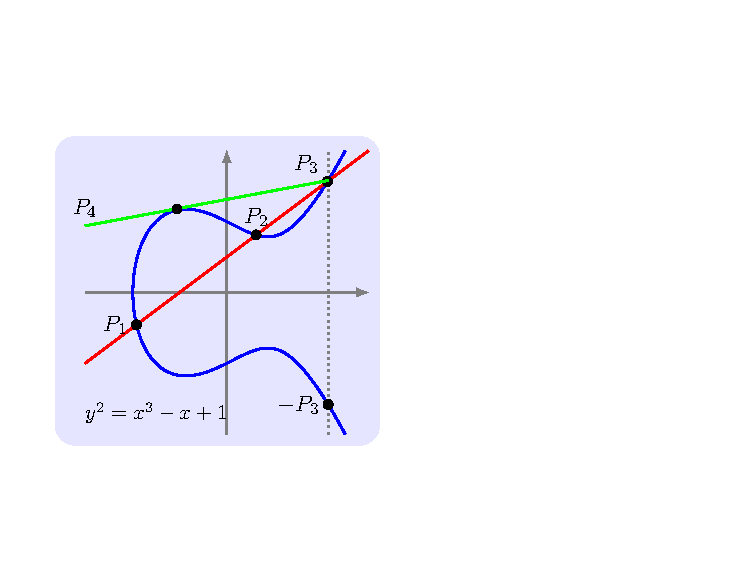
\includegraphics[width=50mm]{pic/ecc.pdf} 
\end{center}
\end{figure}
\end{column}
\begin{column}{5cm}
Every line intersects the curve in 3 points:
\begin{itemize}
\item count twice if tangent.
\item count $\mathcal{O}$ at the vertical infinity of $y$-axis.
\end{itemize}
``\textbf{Addition}'' on points:
\begin{itemize}
\item $P+\mathcal{O} = \mathcal{O} + P = P$.
\item If $P_1, P_2, P_3$ are co-linear, then $P_1 + P_2 + P_3 = \mathcal{O}$.
\end{itemize}
\end{column}
\end{columns}
Some equations: \newline
$-P=(x,-y)$, $P_1 + P_2 = -P_3$, $2P_4=-P_3$, $dP = P + (d-1)P$
\[\text{Key generation:} sk = (P,d); pk = (P,Q=dP)\]
\end{frame}
\begin{frame}\frametitle{A Toy Example of ECDHKE}
\begin{exampleblock}{What is the key?\footnote{The example is generated from https://graui.de/code/elliptic2/}}
In ECDHKE protocol, Alice sends $aP$, Bob sends $bP$, and the key is $(a\cdot b)P$. Alice generates $P=(3,4), a=4$ and receive $(2,7)$.
\end{exampleblock}
\begin{figure}
\begin{center}
\begin{tikzpicture}[scale=0.5,
every node/.style={scale=0.6}, 
every label/.style={blue},
dot/.style={inner sep=1pt, minimum width=5pt, circle, fill=red}]

%\draw (0,0) rectangle (10,10);
\draw[step=1cm,gray!50, thin] (0,0) grid (10,10);

%\node (p\i) at (3,4) [inner sep=1pt, minimum width=2pt, circle, fill=blue] {};


\draw [-latex,thin,red] (3,4)
\foreach \p in {(3,4), (6,4), (2,7), (4,10), (7,5), (10,8), (10,3), (7,6), (4,1), (2,4), (6,7), (3,7)}
{ -- \p };

\draw [-latex,thin,blue] (2,7)
\foreach \p in {(10,8),(4,1),(3,7)}
{-- \p };




 \foreach \p in {(3,4), (6,4), (2,7), (4,10), (7,5), (10,8), (10,3), (7,6), (4,1), (2,4), (6,7), (3,7)}
 { %\node at \p [dot, label=250:{\textbf{\p}}] {}; 
 %\node at \p + (0.2,-0.2) [fill=white] {\p}; 
 \node at \p [dot] {}; 
 }

 \foreach \p in {1,2,3,4,5,6,7,8,9,10} {
 \node at ($\p*(1cm,0) + (0,-0.1cm)$)  {\p}; 
 \node at ($\p*(0,1cm) + (-0.1cm,0)$)  {\p};}
 %\node at \p + (0.2,-0.2) [fill=white] {\p}; 
 
%\node at (3,4) [minimum width=7pt, circle, red, fill=red, draw] {};
%\node at (7,6) [inner sep=1pt, minimum width=7pt, circle, blue, draw] {};
%\node at (10,8) [minimum width=7pt, circle, purple, draw] {};


\node at (7.8,1) [fill=white] {\large $y^2 = x^3 + 3x + 2 \mod 11 $};

% \foreach \i / \p in { 1 / (3,4), 2 / (6,4), 3 / (2,7), 4 / (4,10), 5 / (7,5), 6 / (10,8), 7 / (10,3),
%     8 / (7,6), 9 / (4,1), 10 / (2,4), 11 / (6,7), 12 / (3,7) }
%  { \node at \p [inner sep=1pt, minimum width=2pt, circle, fill=blue] {}; }

% \node (seed) at (-2,0) [draw=red!70,fill=red!20, inner sep=1pt, minimum width=8pt, circle, label=above:$G(s)$] {};

% \foreach \i in {0,1,...,20}
%     {
%     \node (p\i) at (rand,rand) [inner sep=1pt, minimum width=2pt, circle, fill=blue] {};
%     \draw[-,very thin,red] (seed) parabola (p\i);
%     }

\end{tikzpicture}
\end{center}
\end{figure}
\end{frame}
\begin{frame}[fragile]\frametitle{Elliptic Curve Cryptosystems in Practices}
TLS 1.3 (RFC8446) standardizes mandatory-to-implement ECC.
\begin{exampleblock}{P256 or secp256r1 for DSA and DHKE}
\begin{itemize}
\item $p := 2^{256}- 2^{224}+2^{192}+2^{96}-1$
\item $y^2 = x^3 - 3x +b$, $b := $ \verb|5ac635d8 aa3a93e7 b3ebbd55| \verb|769886bc 651d06b0 cc53b0f6 3bce3c3e 27d2604b|
\item It is not clear how $b$ is designed. NOT \textbf{twist secure} as the DLP in its twist is not hard.
NSA implemented a backdoor into the P256 curve based Dual\_EC\_DRBG algorithm.
\end{itemize}
\end{exampleblock}
\begin{exampleblock}{Curve25519 for DHKE}
    \begin{itemize}
    \item $p := 2^{255} - 19$
    \item $y^2 = x^3 + 486662\cdot x^2 +x$  (Montgomery curve)
    \item The curve is generated by a point $P = (9, y)$
    \item It is twist secure and more understandable than P256. And 486662 is a \emph{nothing-up-my-sleeve number}
    \end{itemize}
    \end{exampleblock}
\end{frame}
\begin{frame}\frametitle{Summary}
\begin{itemize}
\item DHKE protocol, ElGamal encryption from CDH, DDH from Discrete Logrithm Problem in prime-order cyclic groups.
\item Elliptic curve cryptography is more efficient and widely used.
\end{itemize}
\end{frame}
\end{document}
